% Options for packages loaded elsewhere
\PassOptionsToPackage{unicode}{hyperref}
\PassOptionsToPackage{hyphens}{url}
%
\documentclass[
]{book}
\usepackage{lmodern}
\usepackage{amssymb,amsmath}
\usepackage{ifxetex,ifluatex}
\ifnum 0\ifxetex 1\fi\ifluatex 1\fi=0 % if pdftex
  \usepackage[T1]{fontenc}
  \usepackage[utf8]{inputenc}
  \usepackage{textcomp} % provide euro and other symbols
\else % if luatex or xetex
  \usepackage{unicode-math}
  \defaultfontfeatures{Scale=MatchLowercase}
  \defaultfontfeatures[\rmfamily]{Ligatures=TeX,Scale=1}
\fi
% Use upquote if available, for straight quotes in verbatim environments
\IfFileExists{upquote.sty}{\usepackage{upquote}}{}
\IfFileExists{microtype.sty}{% use microtype if available
  \usepackage[]{microtype}
  \UseMicrotypeSet[protrusion]{basicmath} % disable protrusion for tt fonts
}{}
\makeatletter
\@ifundefined{KOMAClassName}{% if non-KOMA class
  \IfFileExists{parskip.sty}{%
    \usepackage{parskip}
  }{% else
    \setlength{\parindent}{0pt}
    \setlength{\parskip}{6pt plus 2pt minus 1pt}}
}{% if KOMA class
  \KOMAoptions{parskip=half}}
\makeatother
\usepackage{xcolor}
\IfFileExists{xurl.sty}{\usepackage{xurl}}{} % add URL line breaks if available
\IfFileExists{bookmark.sty}{\usepackage{bookmark}}{\usepackage{hyperref}}
\hypersetup{
  pdftitle={CH10137 Thermodynamics},
  pdfauthor={Fiona Dickinson},
  hidelinks,
  pdfcreator={LaTeX via pandoc}}
\urlstyle{same} % disable monospaced font for URLs
\usepackage{longtable,booktabs}
% Correct order of tables after \paragraph or \subparagraph
\usepackage{etoolbox}
\makeatletter
\patchcmd\longtable{\par}{\if@noskipsec\mbox{}\fi\par}{}{}
\makeatother
% Allow footnotes in longtable head/foot
\IfFileExists{footnotehyper.sty}{\usepackage{footnotehyper}}{\usepackage{footnote}}
\makesavenoteenv{longtable}
\usepackage{graphicx,grffile}
\makeatletter
\def\maxwidth{\ifdim\Gin@nat@width>\linewidth\linewidth\else\Gin@nat@width\fi}
\def\maxheight{\ifdim\Gin@nat@height>\textheight\textheight\else\Gin@nat@height\fi}
\makeatother
% Scale images if necessary, so that they will not overflow the page
% margins by default, and it is still possible to overwrite the defaults
% using explicit options in \includegraphics[width, height, ...]{}
\setkeys{Gin}{width=\maxwidth,height=\maxheight,keepaspectratio}
% Set default figure placement to htbp
\makeatletter
\def\fps@figure{htbp}
\makeatother
\setlength{\emergencystretch}{3em} % prevent overfull lines
\providecommand{\tightlist}{%
  \setlength{\itemsep}{0pt}\setlength{\parskip}{0pt}}
\setcounter{secnumdepth}{5}
\usepackage{booktabs}
\usepackage{amsthm}
\makeatletter
\def\thm@space@setup{%
  \thm@preskip=8pt plus 2pt minus 4pt
  \thm@postskip=\thm@preskip
}
\makeatother
\usepackage[]{natbib}
\bibliographystyle{apalike}

\title{CH10137 Thermodynamics}
\author{Fiona Dickinson}
\date{2020-11-03}

\begin{document}
\maketitle

{
\setcounter{tocdepth}{1}
\tableofcontents
}
\hypertarget{welcome}{%
\chapter*{Welcome}\label{welcome}}
\addcontentsline{toc}{chapter}{Welcome}

The notes have been prepared in a package called BookDown for RStudio so that the equations are accessible to screen readers. However, by providing the notes as a .html webpage I can also embed short videos to further describe some of the topics. If you want videos on any topic please ask and I will do my best to produce the most requested ones.

Further you can download the notes in a format that suits you (either pdf or epub) to view offline, or change the way this document appears for ease of reading.

This document is written in markdown, and particularly in equations typos can creep in. If you spot any typos or think there are any errors please let me know and I will do my best to fix them.

\hypertarget{notes-and-workshops-for-ch10137}{%
\section*{Notes and Workshops for CH10137}\label{notes-and-workshops-for-ch10137}}
\addcontentsline{toc}{section}{Notes and Workshops for CH10137}

This `book' will be updated weekly with content and embedded `micro lecture' video content.

Questions and answers will be provided and some answers will include `process' as well as answer. Please contact me if you need help. Questions on later topics will rely on earlier knowledge.

I am using this format as it is an accessible format. However I have moved over to this format this year and so I would appreciate you pointing out any areas of confusion or where error may have crept in.

\hypertarget{recommended-text}{%
\section*{Recommended text}\label{recommended-text}}
\addcontentsline{toc}{section}{Recommended text}

There is no single recommended text for this section of the course because multiple books can offer valuable extra insight. It may be useful for you to refer to any of the following:

\href{https://bath-ac-primo.hosted.exlibrisgroup.com/primo-explore/search?query=any,contains,Elements\%20of\%20physical\%20chemistry\&tab=local\&sortby=date\&vid=44BAT_VU1\&facet=frbrgroupid,include,978286819\&offset=0\&pcAvailability=false}{The Elements of Physical Chemistry}

\href{https://bath-ac-primo.hosted.exlibrisgroup.com/primo-explore/search?query=any,contains,physical\%20chemistry\%20de\%20paula\&tab=local\&search_scope=CSCOP_44BAT_DEEP\&sortby=date\&vid=44BAT_VU1\&facet=frbrgroupid,include,978327499\&offset=0\&pcAvailability=false}{Atkins' Physical Chemistry}

\href{https://bath-ac-primo.hosted.exlibrisgroup.com/primo-explore/search?query=any,contains,chemistry3\&tab=local\&search_scope=CSCOP_44BAT_DEEP\&sortby=date\&vid=44BAT_VU1\&facet=frbrgroupid,include,978293871\&offset=0\&pcAvailability=false}{Chemistry\textsuperscript{3}}

\hypertarget{version-history}{%
\section*{Version history}\label{version-history}}
\addcontentsline{toc}{section}{Version history}

Week2part1 finished 311020

Degrees of freedom section added to week1part1, week1part2 finished 29th October 2020

Week1Part2 started 28th October 2020.

The initial commit of this book is dated 16th October 2020.

\hypertarget{ch:Part1}{%
\chapter{Week 1 - Part 1: Preliminaries}\label{ch:Part1}}

The `content' videos are all very short, any equations or important images are contained in the text of this document and so pdf slides will not be shared (as these are not an accessible document).

\hypertarget{sec:whyjustwhy}{%
\section{Why thermodynamics matters}\label{sec:whyjustwhy}}

The laws of thermodynamics are some of the most fundamental laws of nature, and in this course I hope you will learn to understand these laws and be able to apply them to explain the world around you.

Thermodynamics is fundamental to the way we live, to our dream of living a better, less impactful life and to how we as `life' work.

\hypertarget{sec:state}{%
\section{State functions - (products - reactants)}\label{sec:state}}

Many properties in thermodynamics are \emph{state functions}, that is properties that only depend upon the current state of the system. State functions are completely independent of the path by which that final state was reached.

Enthalpy (H) is a state function, as are entropy (S), internal energy (U), Gibbs' free energy (G), Helmholtz free energy (F), temperature (T), pressure (p), and chemical composition.

Path functions are unlike state functions in that they depend on the path taken to determine their value.
Heat (q) and work (w) are both examples of path functions.

\begin{itemize}
\item
  Internal energy, U The internal energy is the sum of all of the kinetic and potential energy contributions of the molecules in the system.
\item
  Enthalpy, H The enthalpy is related to the internal energy, but also takes into account any expansion work done by the system, formally ΔH = ΔU + Δ(pV).
\item
  Entropy, S The entropy is a measure of the number of possible arrangements of a system (multiplicity, Ω), formally S = k\textsubscript{B} ln Ω
\item
  Gibbs' free energy, G The Gibbs' free energy is a measure of the energy available to `do work' in a reaction system. It accounts for both the enalpic and entropic contributions of the reaction. ΔG = ΔH − TΔS
\end{itemize}

\begin{figure}

{\centering 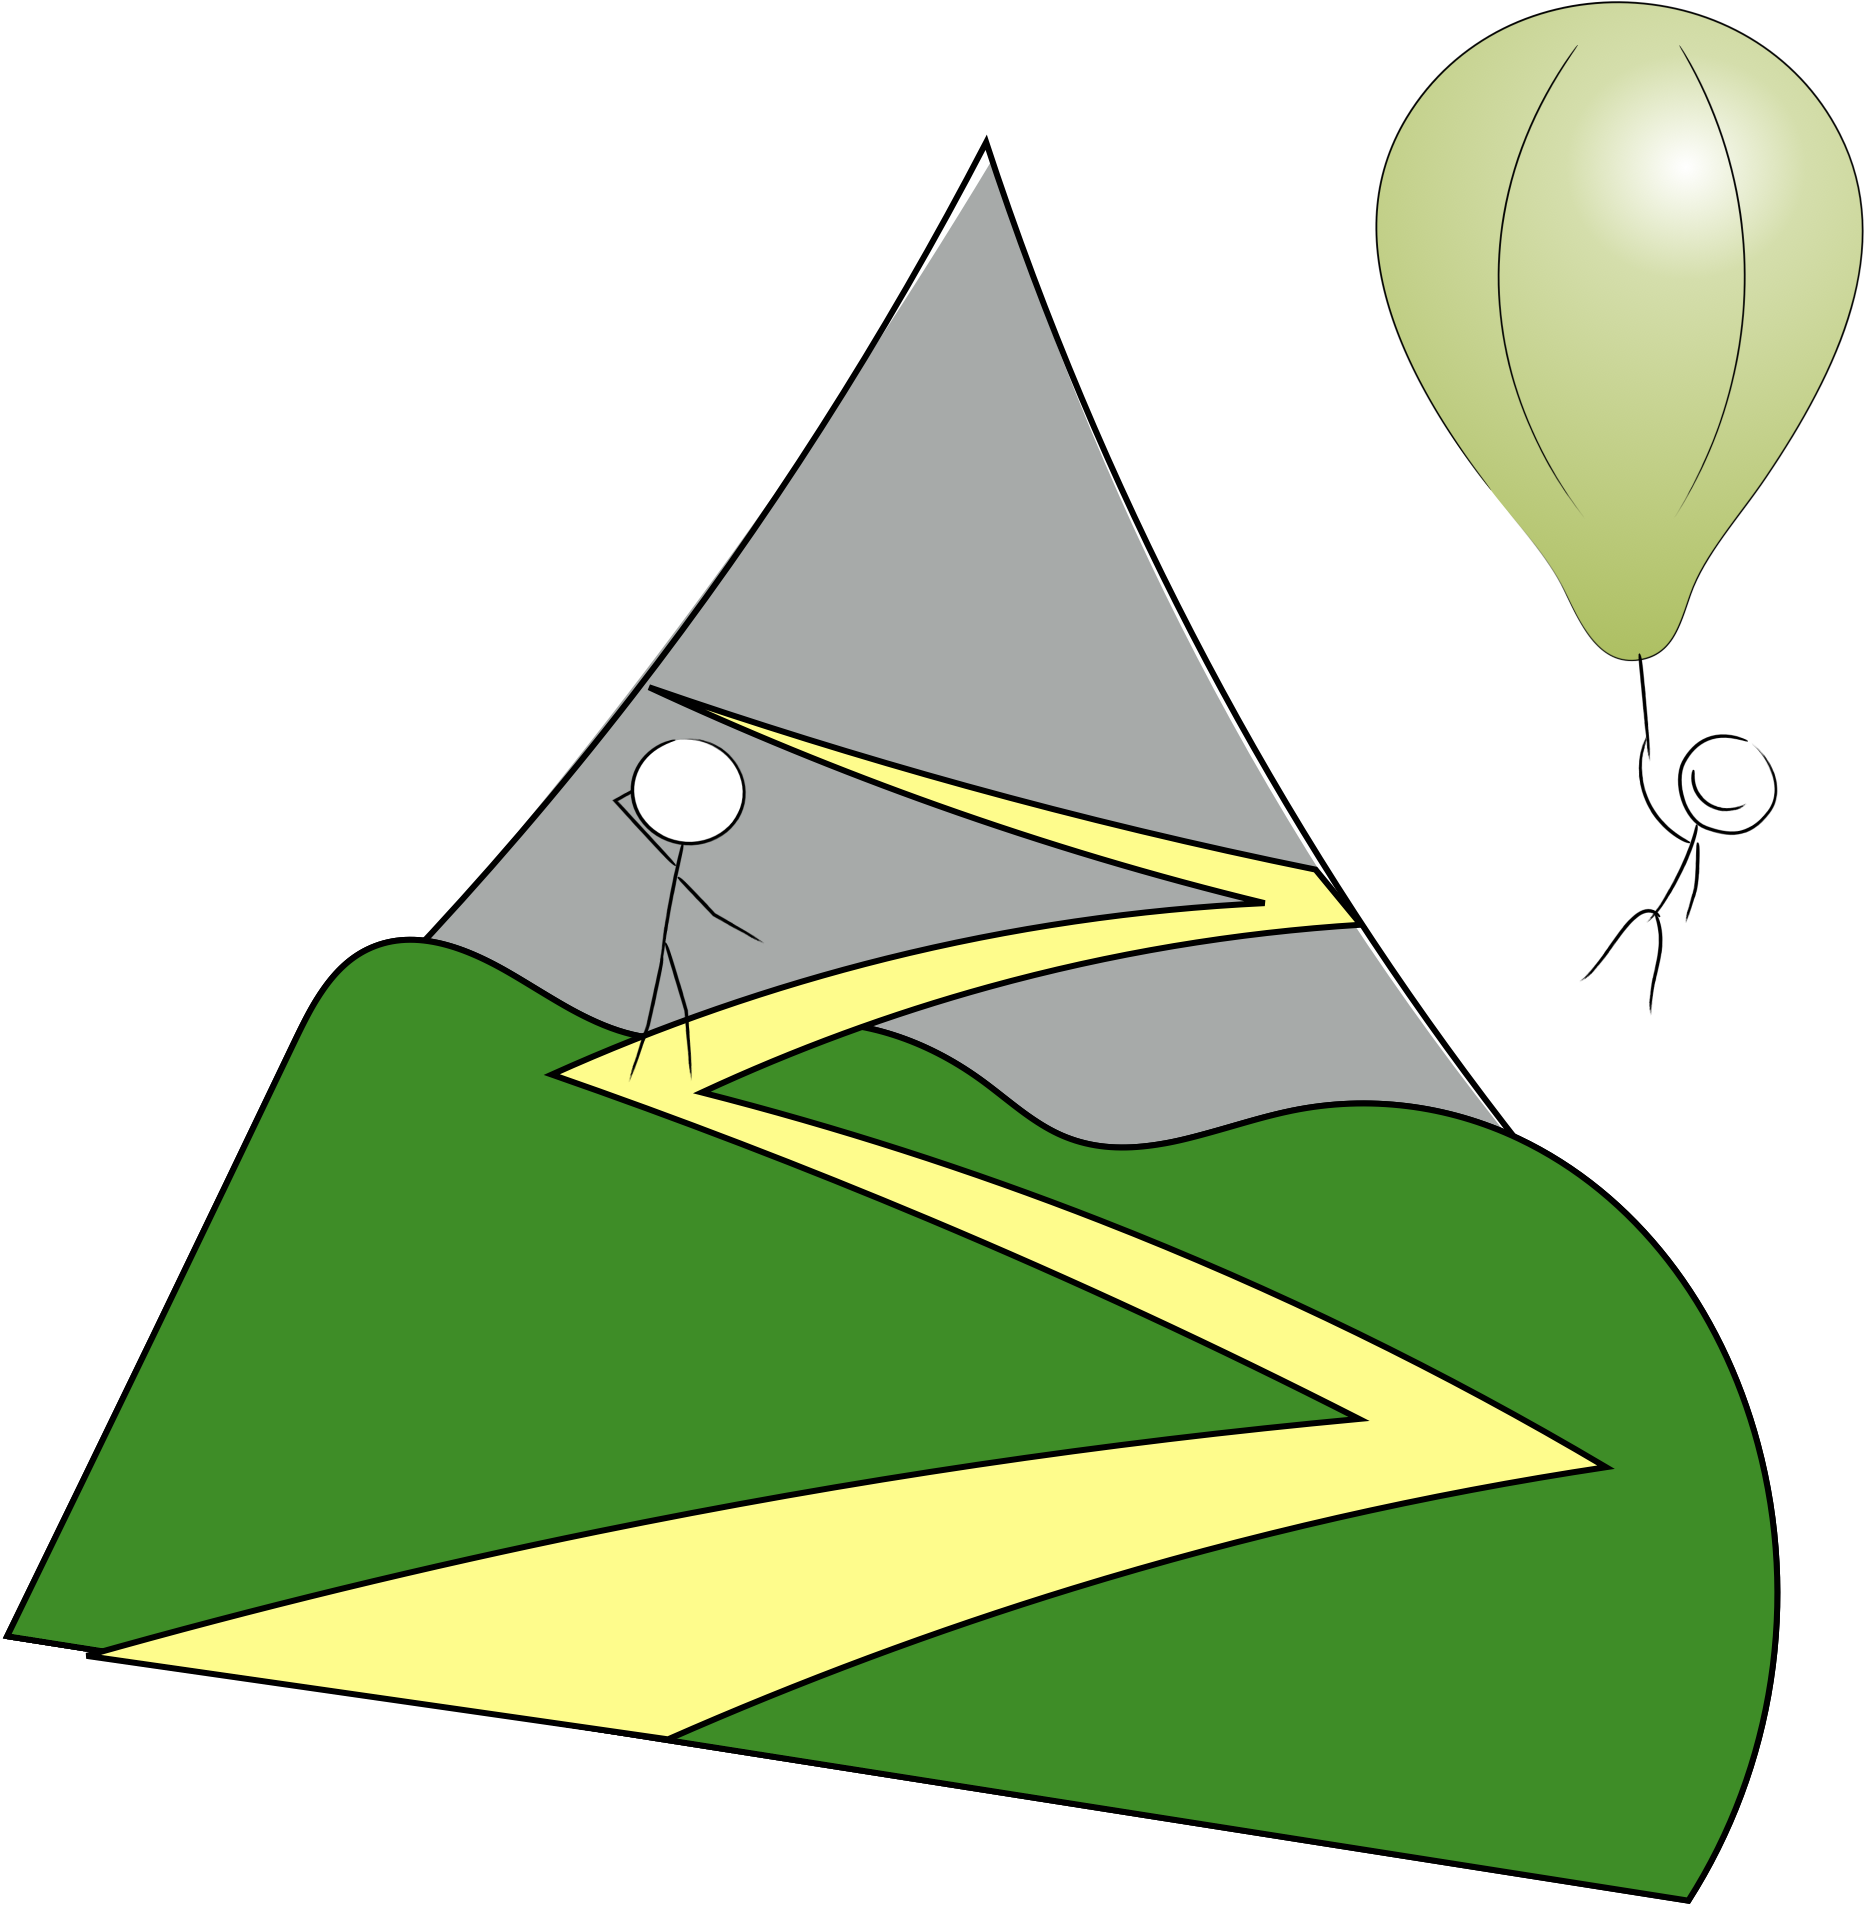
\includegraphics[width=0.3\linewidth]{images/mountain} 

}

\caption{State functions - no matter how you got here, here you are… …altitude is a good analogy for a state function, whether climbing the mountain or flying on the balloon if your altitude is 1000 m it is 1000 m!.}\label{fig:mountain}
\end{figure}

\hypertarget{sec:equations1}{%
\subsection{Useful equations - State functions}\label{sec:equations1}}

Hess' Law (Equation \eqref{eq:enthalpystate}) is something most will be familiar with already. You should try to think about it in terms of an equation however, not the cylces of which you may already be familiar.

\begin{equation}
\Delta_r H^{\ominus} = \sum_{products}v \Delta H^{\ominus}_\textrm{X}-\sum_{reactants}v \Delta H^{\ominus}_\textrm{X}
\label{eq:enthalpystate}
\end{equation}

Similar equations can be used for heat capacity (Equation \eqref{eq:heatcapacitystate}), this equation for heat capacity will then be used later in the course when we look at the effect of temperature on the enthalpy and entropy of reaction.

\begin{equation}
\Delta_r C_p^{\ominus} = \sum_{products}vC_{p,n}^{\ominus}-\sum_{reactants}vC_{p,n}^{\ominus}
\label{eq:heatcapacitystate}
\end{equation}

Entropy, just like enthalpy is a state function.

\begin{equation}
\Delta_r S^{\ominus} = \sum_{products}v S^{\ominus}-\sum_{reactants}v S^{\ominus}
\label{eq:entropystate}
\end{equation}

As is Gibbs' free energy.

\begin{equation}
\Delta _ r G^\ominus = \sum_{prod} v G_n^\ominus - \sum_{react} v  G_n^\ominus 
\label{eq:Gibbsstate}
\end{equation}

The value of each of these variables is independent of the path used to form them. Hence, the same \emph{`products − reactants'} approach always works!

\hypertarget{sec:typesofsystem}{%
\section{Types of thermodynamic system}\label{sec:typesofsystem}}

When we consider anything in thermodynamics we have to consider both the system and its surroundings. The relationship between the system and the surroundings defines the different types of thermodynamic system.

\hypertarget{subsec:isolated}{%
\subsection{Isolated system}\label{subsec:isolated}}

\begin{figure}

{\centering 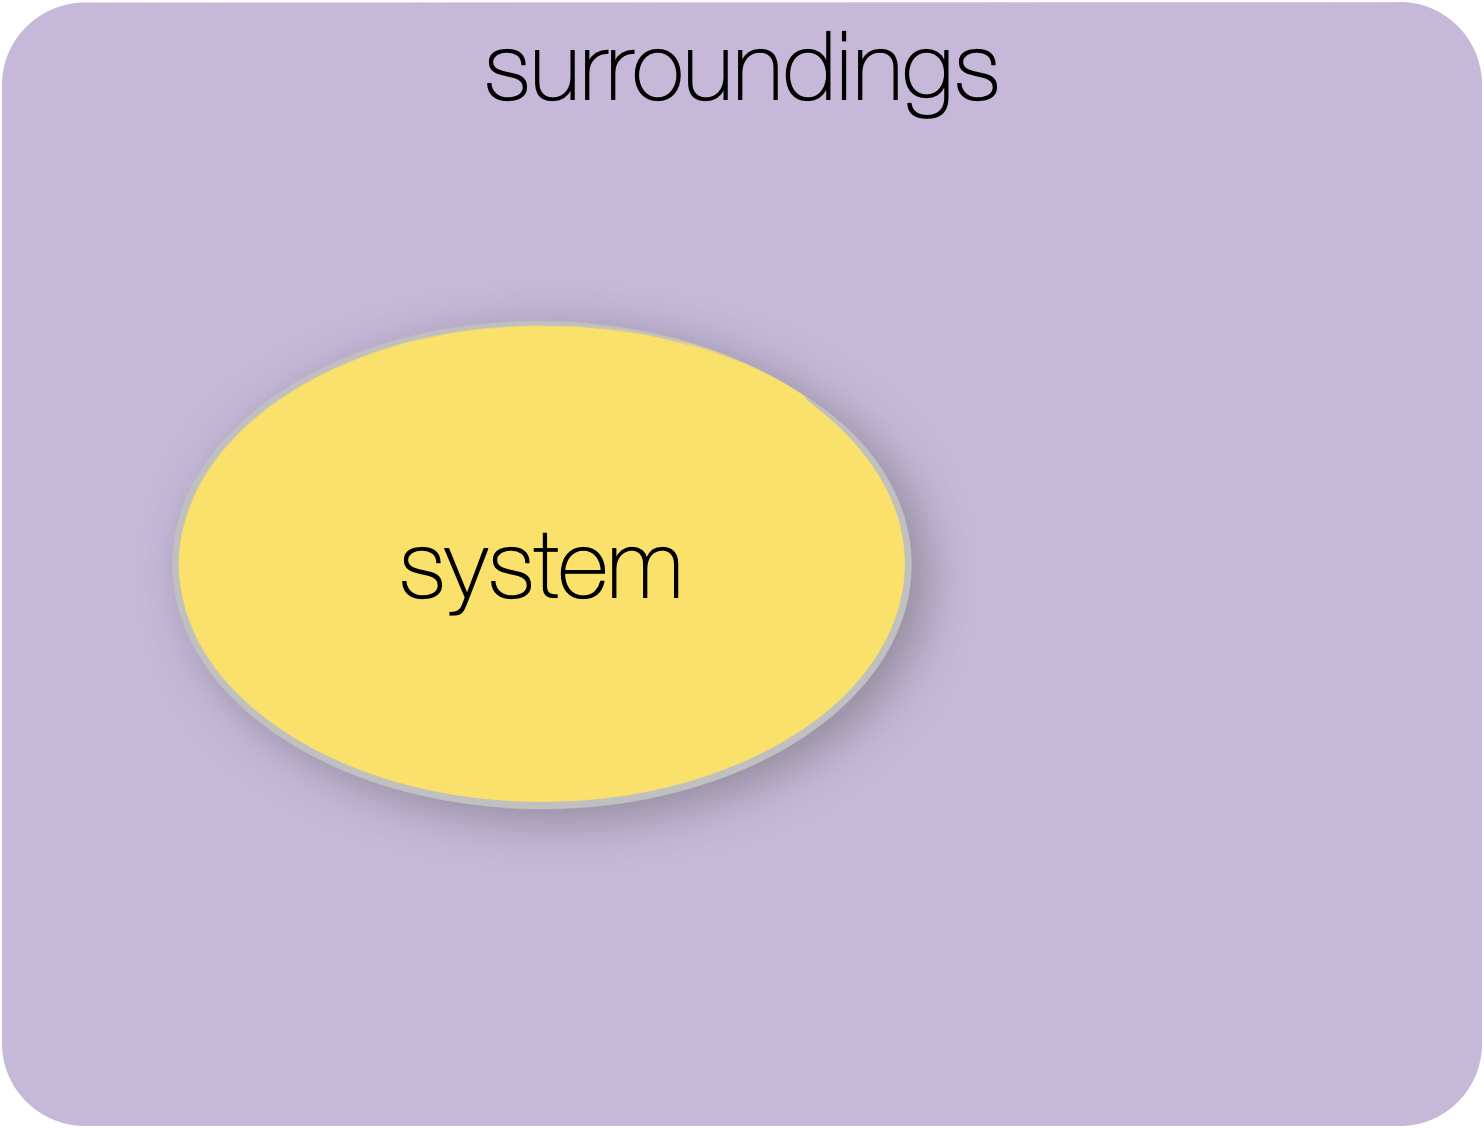
\includegraphics[width=0.3\linewidth]{images/isolated} 

}

\caption{Isolated system: there is no exchange of matter or energy between the system and surroundings.}\label{fig:isolated}
\end{figure}

In an isolated system, there can be no exchange of either matter or energy in any form between the system and surroundings.

A stoppered perfectly insulated flask may be thought of as an isolated system.

\hypertarget{subsec:open}{%
\subsection{Open system}\label{subsec:open}}

\begin{figure}

{\centering 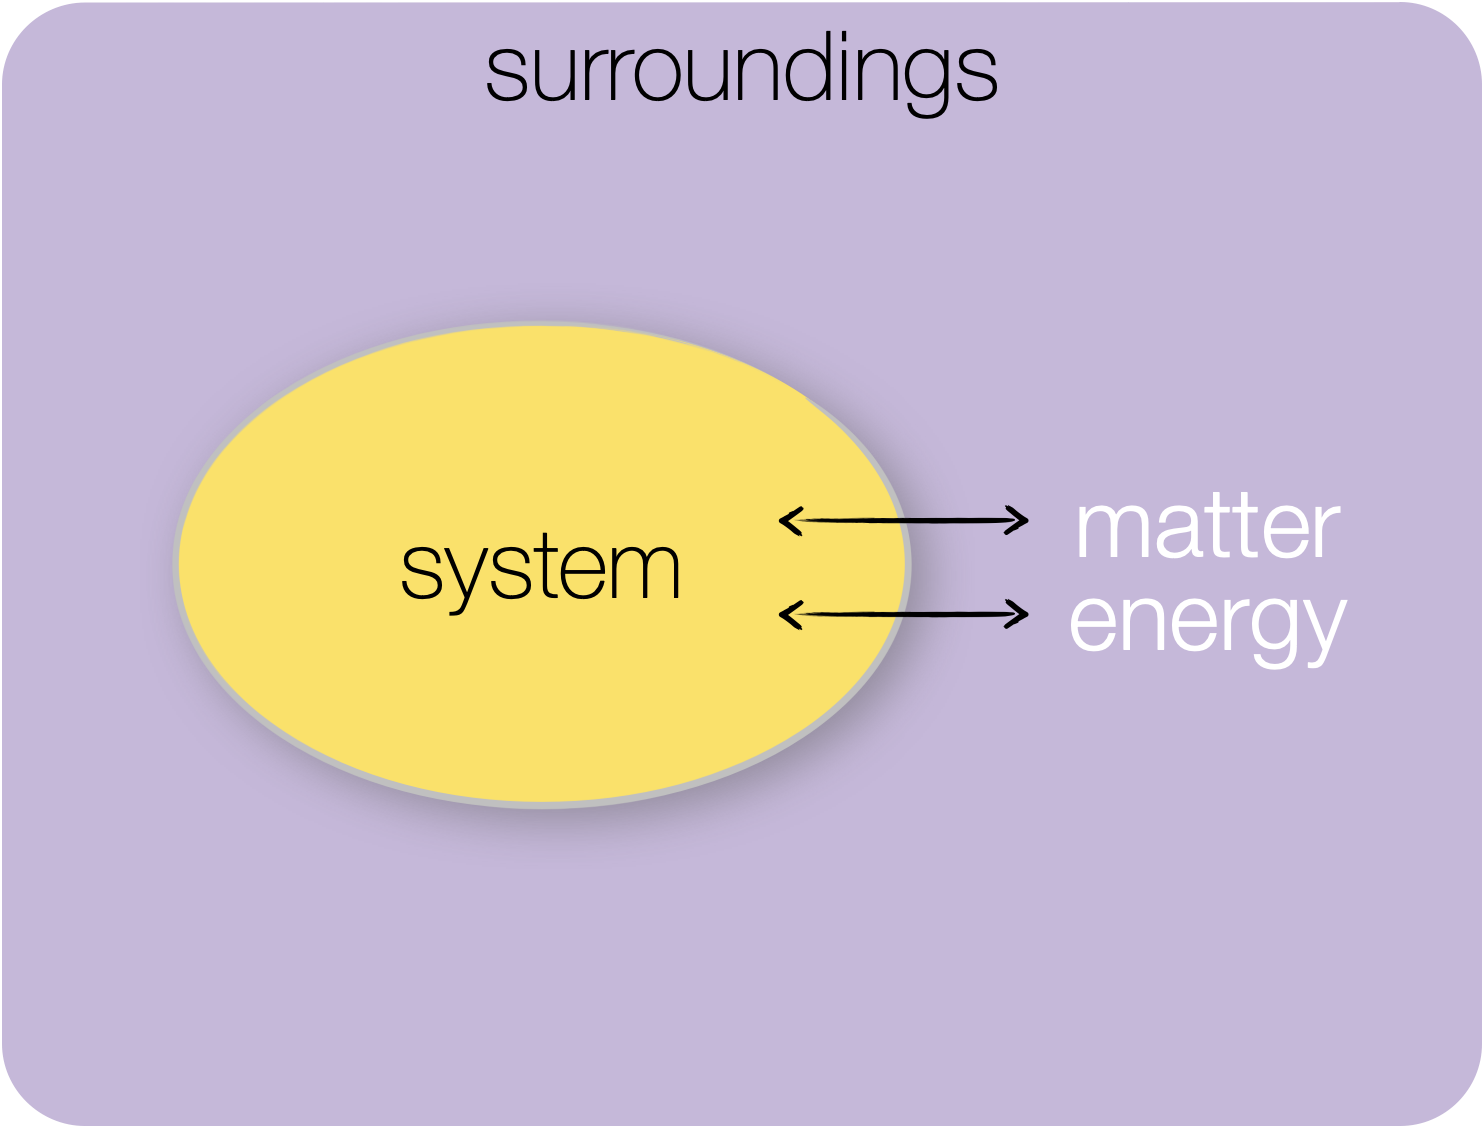
\includegraphics[width=0.3\linewidth]{images/open} 

}

\caption{Open system: in an open system both matter and energy may be exchanged between the system and surroundings.}\label{fig:open}
\end{figure}

In an open system both matter and energy can be exchanged between the system and surroundings.

A cup of tea is a nice example of an open system you can add sugar (if you are weird), drink it, or forget about it and find it cold 2 hours later.

\hypertarget{subsec:closed}{%
\subsection{Closed system}\label{subsec:closed}}

\begin{figure}

{\centering 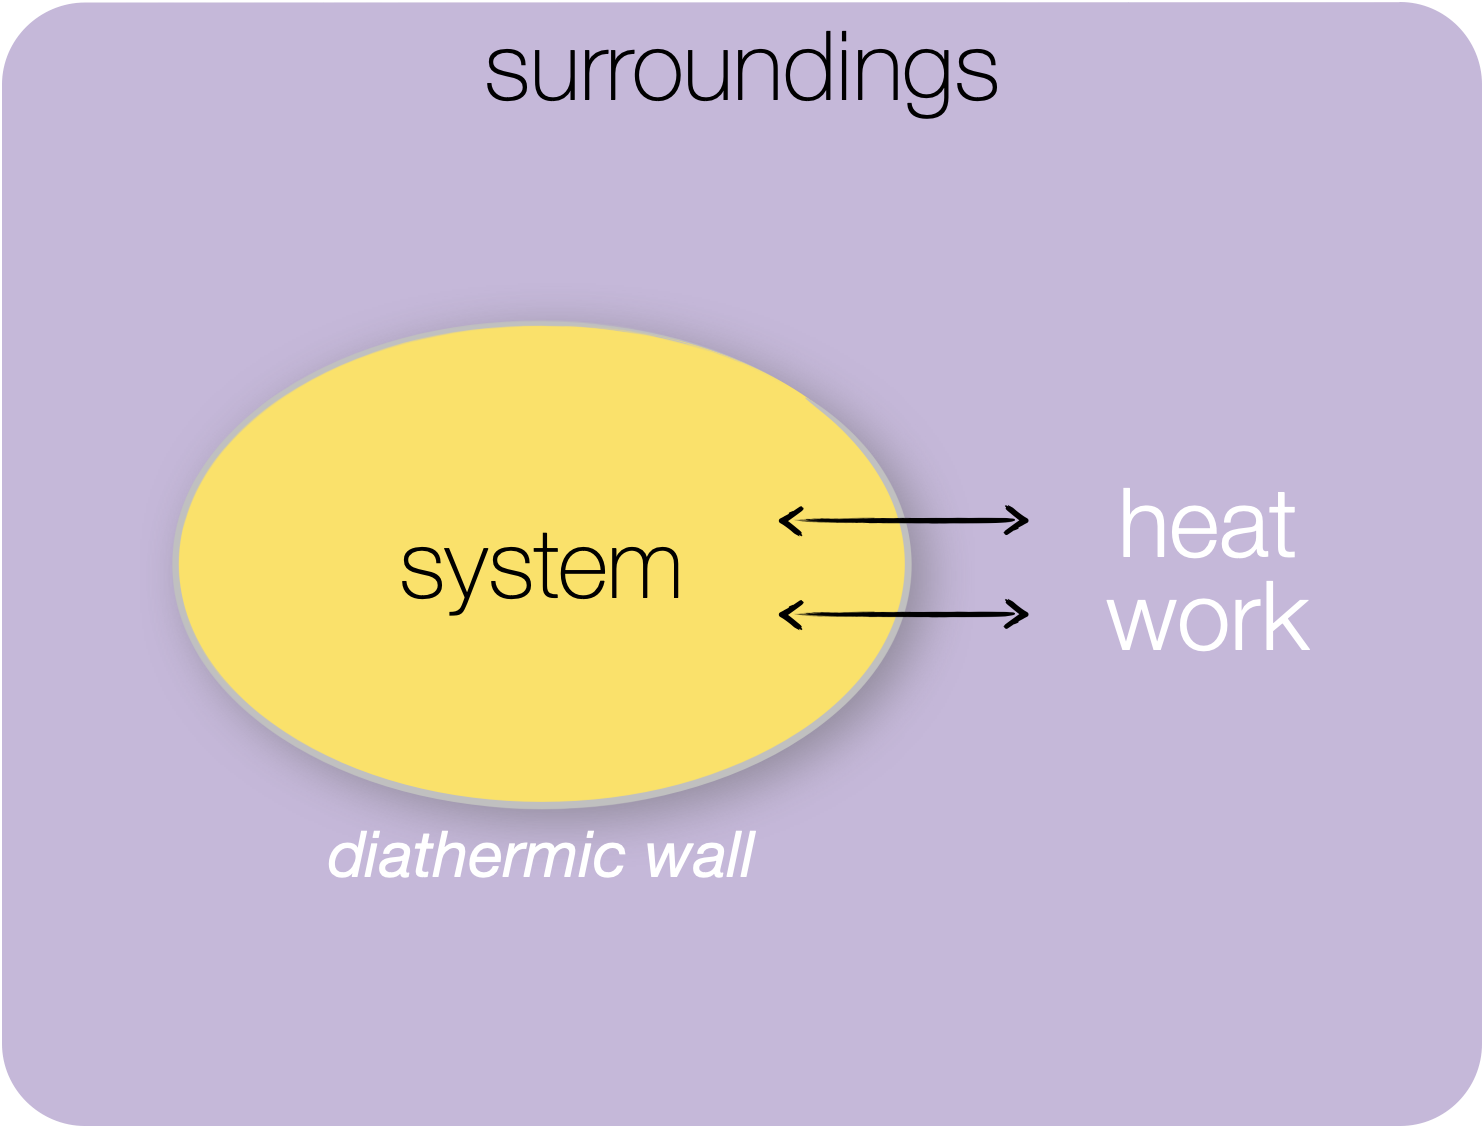
\includegraphics[width=0.3\linewidth]{images/closed} 

}

\caption{Closed system: in a closed system only energy in either the form of heat or work may be exchanged between system and surroundings..}\label{fig:closed}
\end{figure}

A closed system is one where you can't exchange matter but energy in the form of either `heat' or `work' can be exchanged between the system and surroundings.

A closed system is often used as a simpler model than an open system - not many things in life actually fit this model perfectly, but most bench chemistry where we can heat a system fits into this model.

\hypertarget{subsec:adiabatic}{%
\subsection{Adiabatic system}\label{subsec:adiabatic}}

\begin{figure}

{\centering 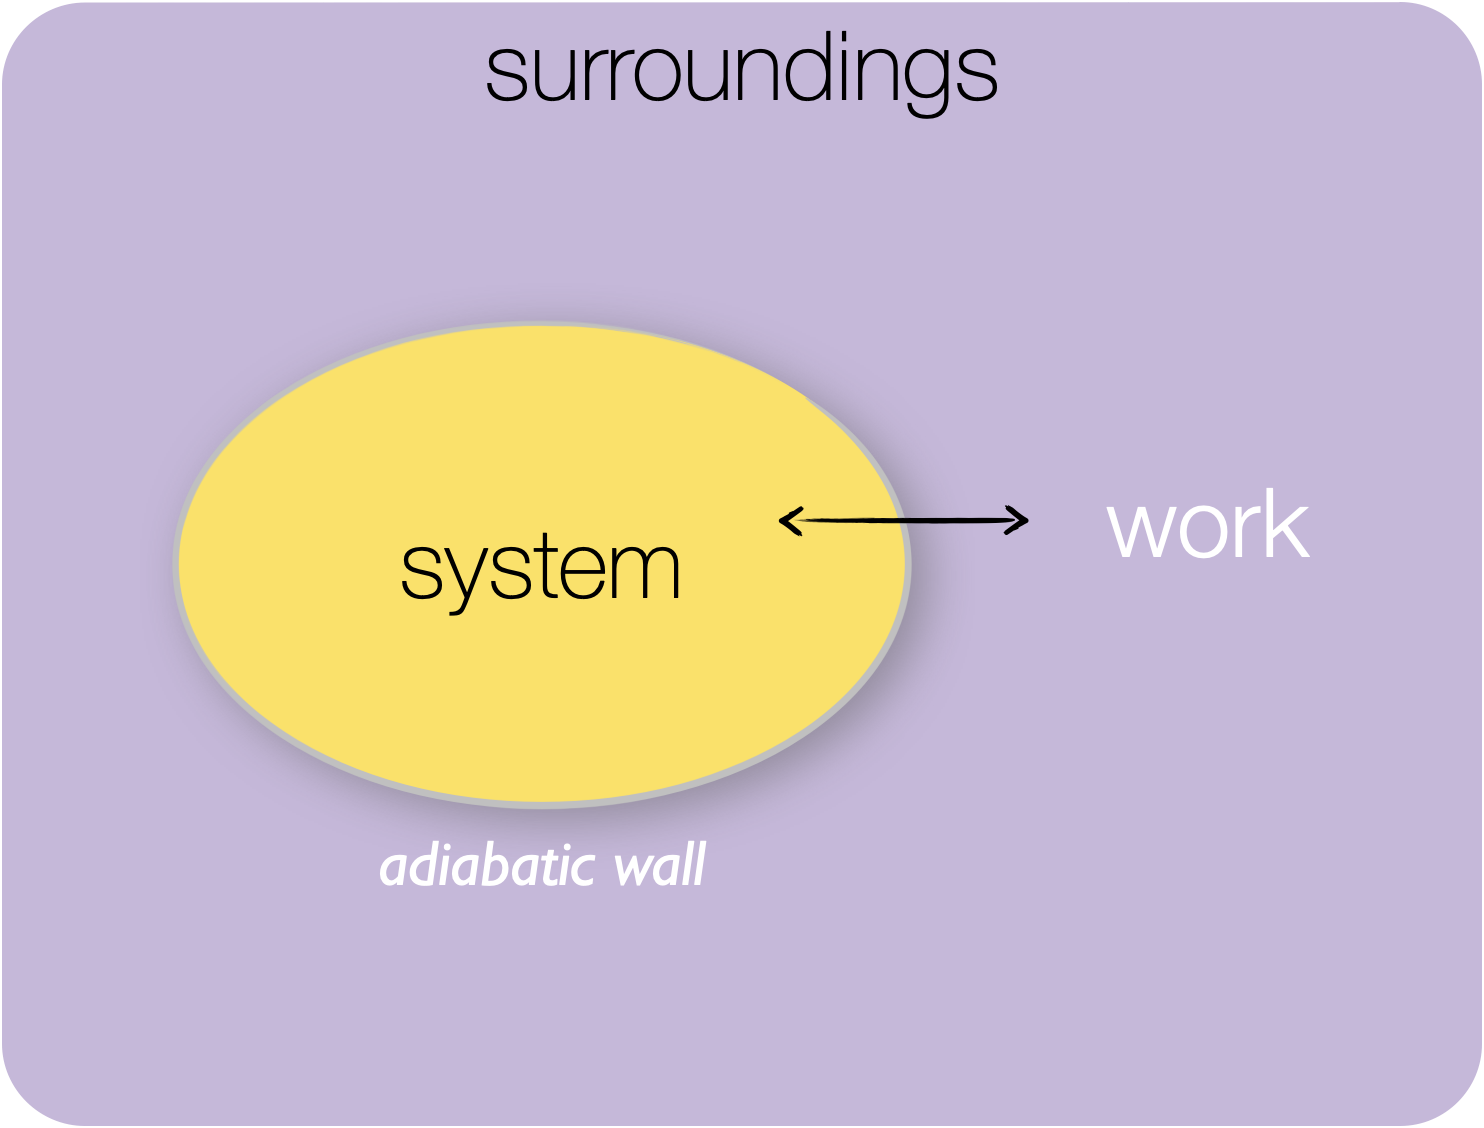
\includegraphics[width=0.3\linewidth]{images/adiabatic} 

}

\caption{Adiabatic system: in an adiabatic system only energy in the form of work may be exchanged between the system and surroundings.}\label{fig:adiabatic}
\end{figure}

An adiabatic system is one where you can't have any flow of heat between the system and surroundings, but you can exchange energy in the form of work.

This would mean that the system is insulated from the surroundings, and therefore the system may not be in thermodynamic equilibrium with the surroundings.

We will learn more about both `heat' and `work' later in the course.

\hypertarget{sec:extensiveintensive}{%
\section{Extensive and intensive properties}\label{sec:extensiveintensive}}

The difference between extensive and intensive properties is whether the property depends upon the amount of `stuff' you have.

\hypertarget{sec:intenstive}{%
\subsection{Intensive properties}\label{sec:intenstive}}

Properties which are \emph{independent} of the amount of stuff are called `intensive properties'.

Temperature is an example of an intensive property as are all of `molar' properties (the quantity of something `per mole'): molar heat capacity, molar enthalpy, molar entropy, molar Gibbs' energy, \emph{etc}\ldots{} in physics the term `specific' is often used such as specific heat capacity and specific enthalpy, these are also intensive properties based on the fixed amount of a `gram' (g).

\hypertarget{sec:extensive}{%
\subsection{Extensive properties}\label{sec:extensive}}

Conversely, properties which are \emph{dependent} on the amount of stuff you have are called extensive properties.

Many intensive properties have extensive equivalents, so whilst we have `molar heat capacity' we also have `heat capacity'; one looks at the amount of energy it takes to raise one mole of a thing by one kelvin, whereas the other looks at how much energy it takes to raise the temperature how ever much of a thing we have by on kelvin.

Consequently extensive properties have different units to their `equivalent' intensive property.

Other examples of extensive properties are unsurprisingly: volume, mass, amount (as in moles), and length.

Whilst knowing the terms extensive and intensive isn't vital it is hugely important to recognise that sometimes terms will appear with different units to suit the particular situation.

\hypertarget{sec:classicalstat}{%
\section{Classical vs.~Statistical thermodynamics}\label{sec:classicalstat}}

Thermodynamics is quite an old subject, much of our understanding of why chemical reactions happen is based in 19th century science. This understanding was based on emperical observation of things like steam engines and battery piles. It scientists trying to understand how things work in order to make them better, make them more efficient, and make them safer.

This 19th century (and earlier) view of the world didn't even consider things we take for granted now, nowhere in thermodynamics do we ever really think about atoms. We talk about ideal systems (those that follow the rules nicely), but never really care about the reaction taking place, it is all just the bulk average behaviour of the system.

Then in the late 19th century Ludwig Boltzmann proposed a different way of thinking about thermodynamics. He started to think about the `average' behaviour of individual atoms. This version of statistical mechanics gave an explanation of what concepts like entropy were and it helped explain macroscopic phenomena (such as pressure and temperature) on an atomic and molecular level.

Statistical thermodynamics started to be able to explain the values of what had until then been emperical constants.

Consequently in this course we will look at thermodynamics from both a classical and statistical point of view.

\hypertarget{degrees-of-freedom}{%
\subsection{Degrees of Freedom}\label{degrees-of-freedom}}

NOTE - I've also added this to the week1 part1 so this section is duplicated.

Perhaps unsurprisingly the structure of molecules is an important concept when we consider thermodynamics from the molecule up perspective, but perhaps surprisingly classical thermodynamics does not care at all the structure of the molecules in the system we are considering.

\begin{figure}

{\centering 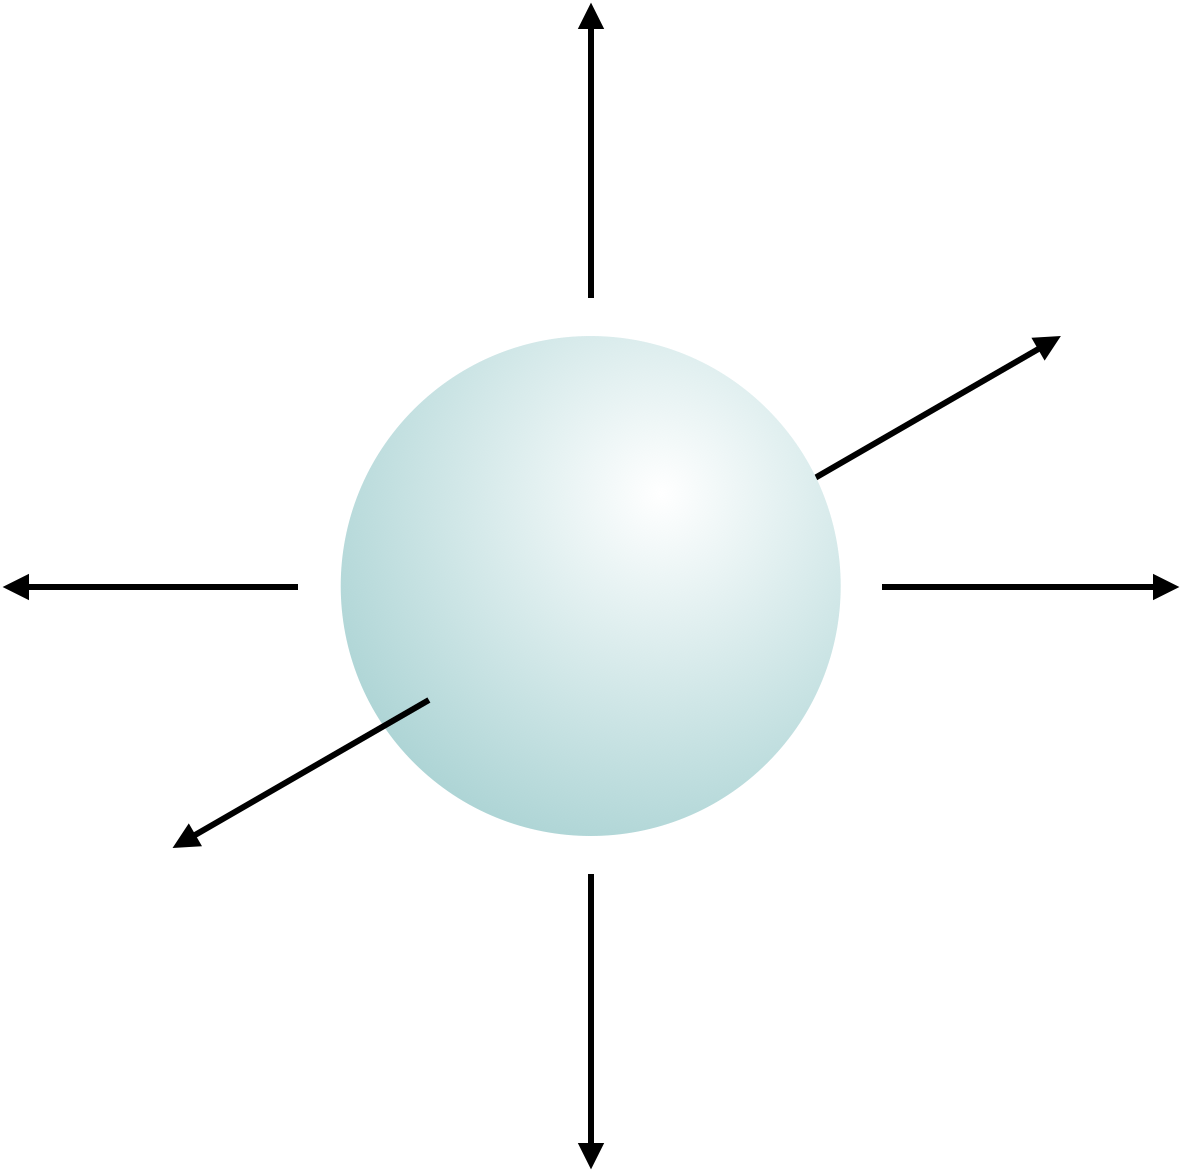
\includegraphics[width=0.8\linewidth]{images/atomdegrees} 

}

\caption{Every atom has three degrees of freedom, these are movement along the x, y and z axis.}\label{fig:atomdegrees}
\end{figure}

When atoms combine to form moleucules the total number of degrees of freedom must be conserved, and so new types of degrees of freedom are introduced, namely molecular rotations and molecular vibrations (figure \ref{fig:typesdegree}, and equations \eqref{eq:lineardof} and \eqref{eq:nonlineardof}).

\begin{figure}

{\centering 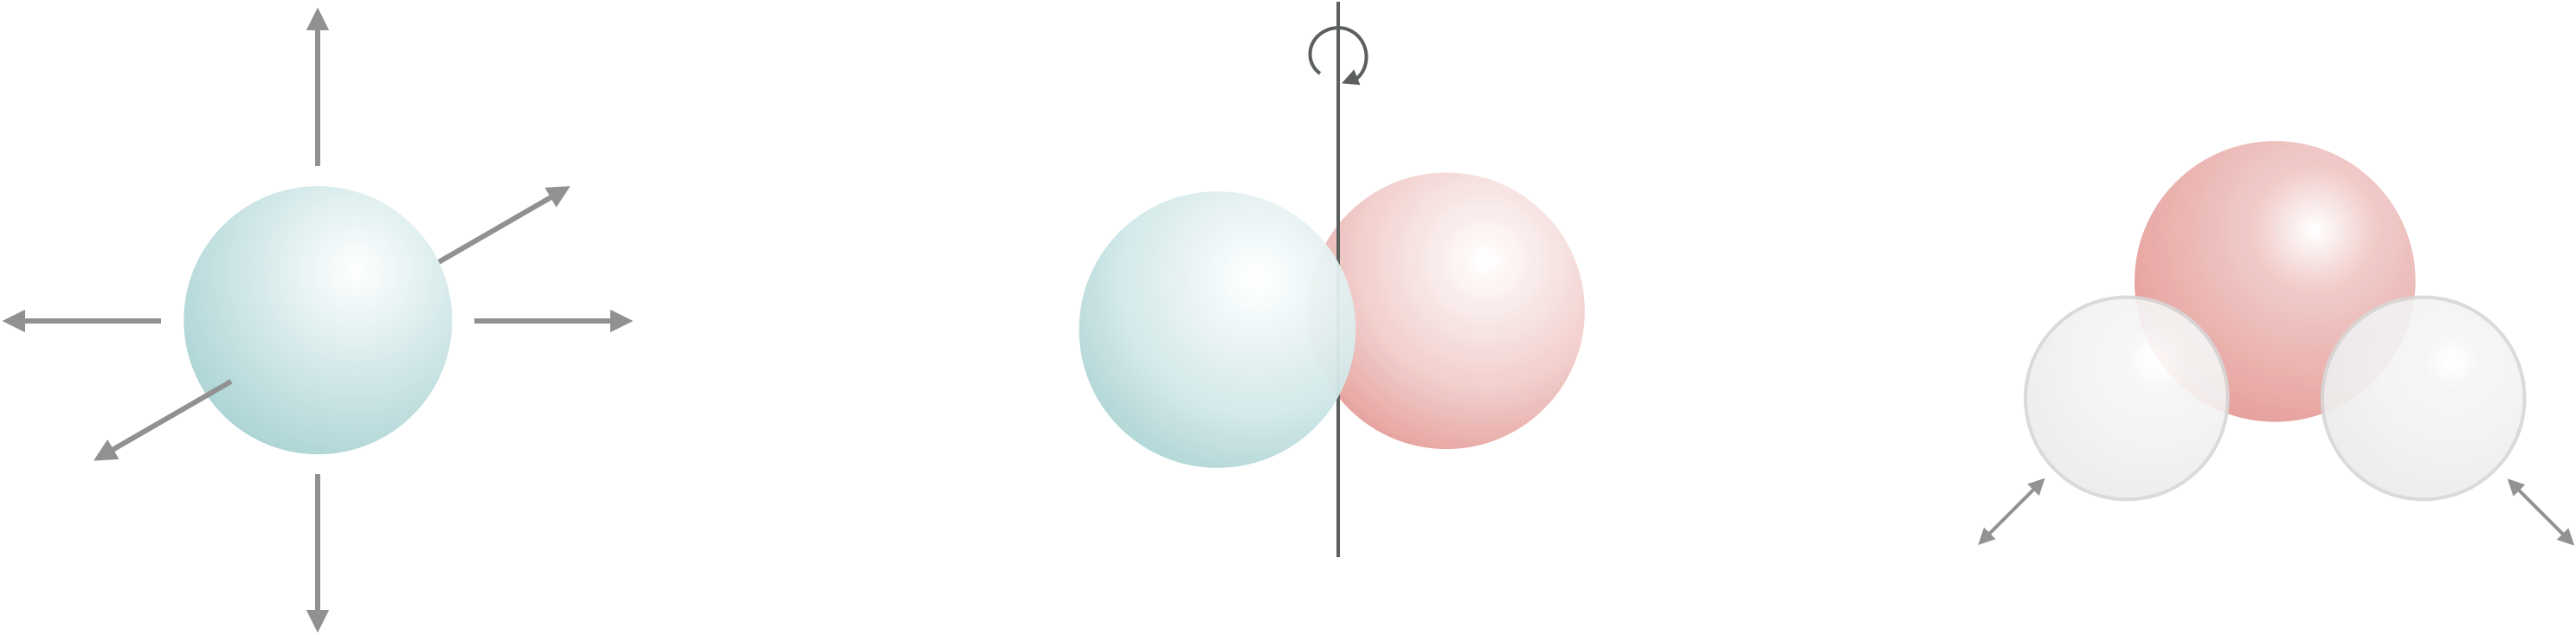
\includegraphics[width=0.8\linewidth]{images/typesdegree} 

}

\caption{Translations, molecular rotations and molecular vibrations are all degrees of freedom.}\label{fig:typesdegree}
\end{figure}

For linear molecules there are three translational degrees of freedom, two rotational degrees of freedom (figure \ref{fig:linear}) and the number of vibrational degrees of freedom is given by equation \eqref{eq:lineardof}, where N is the total number of atoms in the molecule:

\begin{equation}
x = 3N-5
\label{eq:lineardof}
\end{equation}

\begin{figure}

{\centering 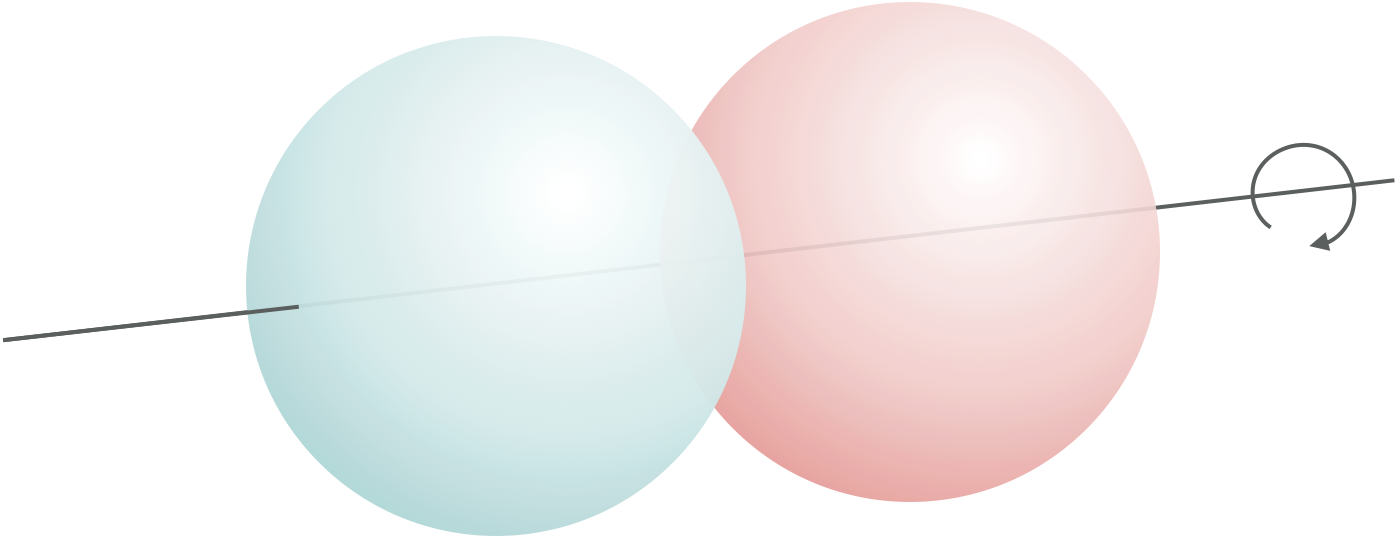
\includegraphics[width=0.8\linewidth]{images/linear} 

}

\caption{In linear molecules there are only two rotational degrees of freedom as rotaion around the z-axis (the long axis of the molecule) are equivalent and therefore dont contribute to the degrees of freedom.}\label{fig:linear}
\end{figure}

For non-linear molecules there are three translational degrees of freedom, three rotational degrees of freedom and the number of vibrational degrees of freedom is given by equation \eqref{eq:nonlineardof}, again where N is the total number of atoms in the molecule:

\begin{equation}
x = 3N-6
\label{eq:nonlineardof}
\end{equation}

\hypertarget{example-calculations}{%
\section{Example calculations}\label{example-calculations}}

\hypertarget{sec:examplehess}{%
\subsection{Example calculation - Hess's Law}\label{sec:examplehess}}

How much energy is released when 4.60 g of sodium reacts with excess water to give NaOH (aq) \& H\textsubscript{2} (g)?

\begin{itemize}
\tightlist
\item
  ΔH\textsubscript{f}\textsuperscript{⦵} NaOH = −425.61 kJ mol\textsuperscript{−1}
\item
  ΔH\textsubscript{f}\textsuperscript{⦵} H\textsubscript{2}O = −285.83 kJ mol\textsuperscript{−1}
\end{itemize}

The enthalpy of formation of elements in their standard state (\emph{e.g.} Na (s) \& H\textsubscript{2} (g)) is zero.

Therefore using equation \eqref{eq:enthalpystate}:

\begin{equation*}
\Delta H_{rxn}^{\ominus}= \Delta H_{f}^{\ominus}(\textrm{NaOH})-\Delta H_{f}^{\ominus}(\textrm{H}_2\textrm{O})= −425.61 \textrm{ kJ mol}^{−1} − −285.83 \textrm{ kJ mol}^{−1} = −139.78 \textrm{ kJ mol}^{−1}
\end{equation*}

\(R_M \textrm{ Na} = 22.989769 \textrm{ g mol}^{−1}\)
Therefore:

\begin{equation*}
n \textrm{(Na)} = \frac{m}{R_M} = \frac{4.60 \textrm{ g}}{ 22.989769 \textrm{ g mol}^{−1}} = 0.200 \textrm{ mol}
\end{equation*}

\emph{note sf!}

Therefore if 4.60g reacts:

\begin{equation*}
\Delta H_{rxn}^⦵ ( \textrm{kJ}) = \Delta H_{rxn}^⦵ ( \textrm{kJ mol}^{−1}) × \textrm{mol} = −139.78 \textrm{kJ mol}^{-1} × 0.200 \textrm{mol} = −28.0 \textrm{ kJ}
\end{equation*}

The `−' sign indicates that heat is released (evolved) and the temperature of the surroundings increases.

\hypertarget{subsec:examplekirchoff}{%
\subsection{Example Calculation - Kirchoff's law}\label{subsec:examplekirchoff}}

Kirchoff's laws may be used to adjust calculated values of enthalpy and entropy of reaction to different temperatures, they use the difference in heat capacity of products and reactants to do this. Determine \(ΔC_{p,m}\) for the following reaction:

CH\textsubscript{3}CH\textsubscript{2}OH (aq) + CH\textsubscript{3}COOH (aq) ⟶ CH\textsubscript{3}COOCH\textsubscript{2}CH\textsubscript{3} (aq) + H\textsubscript{2}O (l)

\begin{longtable}[]{@{}cc@{}}
\toprule
& \(ΔC_{p,m}\) / J K\(^{−1}\) mol\(^{−1}\)\tabularnewline
\midrule
\endhead
CH\textsubscript{3}CH\textsubscript{2}OH (aq) & 111.46\tabularnewline
CH\textsubscript{3}COOH (aq) & 124.3\tabularnewline
CH\textsubscript{3}COOCH\textsubscript{2}CH\textsubscript{3} (aq) & 170.1\tabularnewline
H\textsubscript{2}O (l) & 33.58\tabularnewline
\bottomrule
\end{longtable}

\begin{equation*}
ΔC_{p,m \textrm{ rxn}} = (C_{p,m} \textrm{CH$_3$COOCH$_2$CH$_3$ (aq)} + C_{p,m} \textrm{H$_2$O (l)}) − (C_{p,m} \textrm{CH$_3$CH$_2$OH (aq)} + C_{p,m} \textrm{CH$_3$COOH (aq)})
\end{equation*}

\begin{equation*}
ΔC_\textrm{p,m rxn} = (170.1 + 33.58) − (111.46 + 124.3) \textrm{ J K$^{-1}$ mol}^{−1}) = − 32.1 \textrm{ J K$^{-1}$ mol}^{−1}
\end{equation*}

\hypertarget{sec:Questions1}{%
\section{Questions}\label{sec:Questions1}}

Later in this course you will learn about the origin of these equations, for now it is enough to be able to balance chemical equations and use the fact that each of the variables in teh following equations are state functions.

\begin{enumerate}
\def\labelenumi{\arabic{enumi}.}
\tightlist
\item
  What is the standard Gibbs' free energy of the oxidation of ammonia (NH\textsubscript{3}) to nitric acid (NO)?
\end{enumerate}

Hint: This is a redox reaction.

\(ΔG^⦵_{f, \textrm{NH}_3} = −16.45 \textrm{ kJ mol}^{−1}\)

\(ΔG^⦵_{f, \textrm{NO}} = +86.55 \textrm{ kJ mol}^{−1}\)

\(ΔG^⦵_{f, \textrm{H}_2 \textrm{O}} = −228.57 \textrm{ kJ mol}^{−1}\)

\begin{center}\rule{0.5\linewidth}{0.5pt}\end{center}

\begin{enumerate}
\def\labelenumi{\arabic{enumi}.}
\setcounter{enumi}{1}
\tightlist
\item
  Methanol fuel cells have been proposed as replacements for internal combustion engines. Methanol (density, ρ = 792 kg m\textsuperscript{−3}) is reacted in a fuel cell to be completely oxidised.
\end{enumerate}

Given the enthalpies of formation required are listed below determine the amount of energy released per mL of methanol.

\(ΔH^⦵_{f, \textrm{CH}_3\textrm{OH}} = −425.61 \textrm{ kJ mol}^{−1}\)

\(ΔH^⦵_{f, \textrm{H}_2 \textrm{O}} = −241.82 \textrm{ kJ mol}^{−1}\)

\(ΔH^⦵_{f, \textrm{CO}_2} = −393.51 \textrm{ kJ mol}^{−1}\)

\begin{center}\rule{0.5\linewidth}{0.5pt}\end{center}

\begin{enumerate}
\def\labelenumi{\arabic{enumi}.}
\setcounter{enumi}{2}
\tightlist
\item
  Ammonium dichromate decomposes upon heating in a spectacular `volcano' reaction:
\end{enumerate}

(NH\textsubscript{4})Cr\textsubscript{2}O\textsubscript{7} (s) ⟶ N\textsubscript{2} (g) + 4 H\textsubscript{2}O (g) + Cr\textsubscript{2}O\textsubscript{3} (s)

Determine the enthalpy of reaction for this process given the following data.

\(ΔH^⦵_{f, \textrm{(NH}_4\textrm{)Cr}_2\textrm{O}_7\textrm{ (s)}} = −1810 \textrm{ kJ mol}^{−1}\)

\(ΔH^⦵_{f, \textrm{H}_2 \textrm{O (g)}} = −240 \textrm{ kJ mol}^{−1}\)

\(ΔH^⦵_{f, \textrm{Cr}_2 \textrm{O}_3 \textrm{ (g)}} = −1140 \textrm{ kJ mol}^{−1}\)

How would the enthalpy of reaction differ if liquid water was formed? Justify your answer.

\hypertarget{sec:Answers1}{%
\section{Answers}\label{sec:Answers1}}

\begin{enumerate}
\def\labelenumi{\arabic{enumi}.}
\tightlist
\item
  \(ΔG_{rxn}^⦵\) = −239.86 kJ mol\textsuperscript{−1}\(_{NH_3}\) (per mole of NH\textsubscript{3})
\item
  \(ΔH_{rxn}^⦵\) = -11.2 kJ cm\textsuperscript{-3}
\item
  \(ΔH_{rxn}^⦵\) = -290 kJ mol\textsuperscript{−1}, become more negative as heat is released upon condensing (we will cover this later in the course if you don't understant this last part, please don't stress).
\end{enumerate}

\hypertarget{ch:Part2}{%
\chapter{Week 1 - Part 2}\label{ch:Part2}}

There are different methods of teaching thermodynamics, many come at the problem from a very mathematical viewpoint, with partial derivatives, and operators. This course does not do that, the emphasis here is on understanding thermodynamic concepts, and being able to apply them solve problems. At no point will I expect you to be able to derive something, and I only include the derivations of a couple of equations where I feel it aids understanding of the concept.

If you wish to see a more mathematical version of this course it is covered in a number of textbooks, including the recommended text for this course, Atkin's Elements of Physical Chemistry.

\hypertarget{zeroth-law-of-thermodynamics}{%
\section{Zeroth Law of Thermodynamics}\label{zeroth-law-of-thermodynamics}}

There are four laws of thermodynamics, each introduces a thermodynamic concept. The first of these laws was actually the last to be defined and is called the \emph{zeroth law}.

The zeroth law deals with the idea of thermal equilibrium, and leads to the concept of \emph{temperature}.

\begin{figure}

{\centering 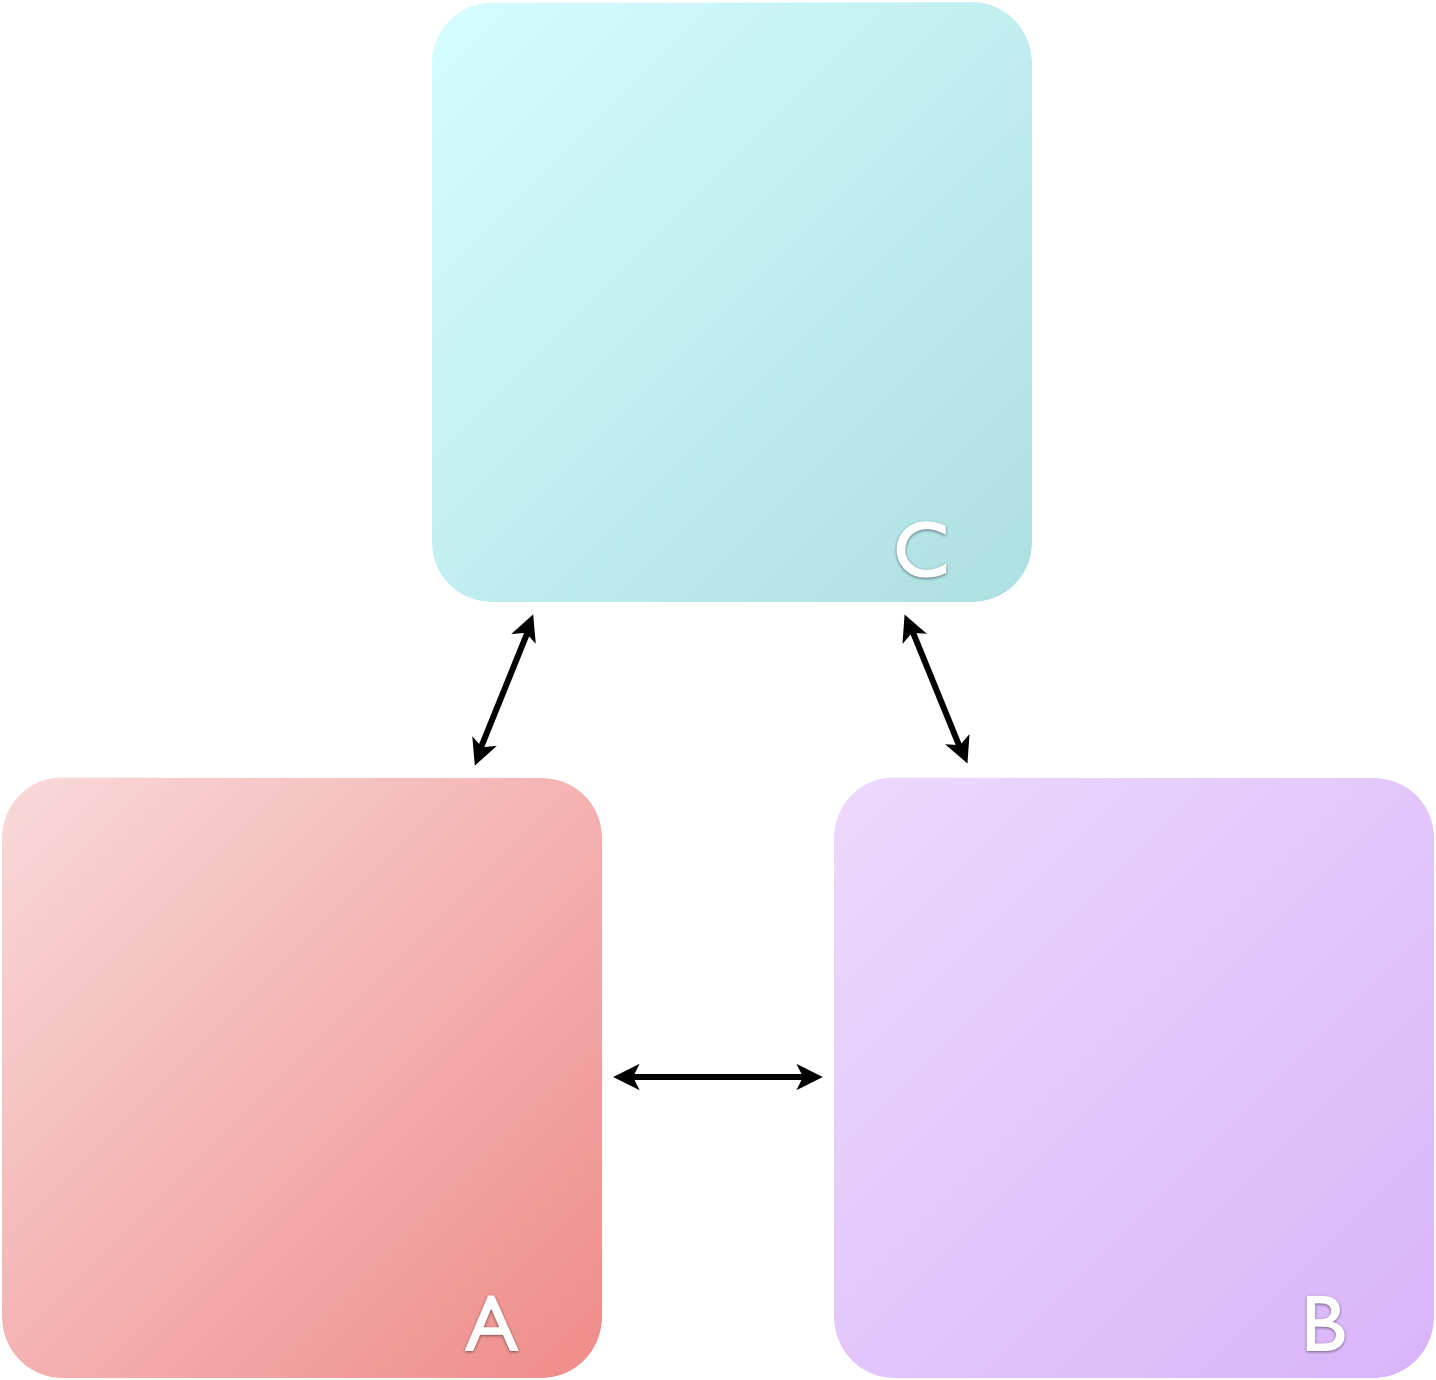
\includegraphics[width=0.5\linewidth]{images/thermalequilibrium} 

}

\caption{The zeroth law of thermodynamics states: if A is in thermal equilibrium with B, and B is in thermal equilibrium with C, then C will be in thermal equilibrium with A.}\label{fig:zerothlaw}
\end{figure}

The thermal equilibrium used in figure @\ref(fig:zerothlaw) basically says that if A and B are in thermal equilibrium then they must have the same temperature. Therefore the first thermodynamic concept we meet is temperature, which has the unit K (kelvin).

\emph{The following video is for context and interest only}

\hypertarget{what-is-temperature}{%
\section{What is temperature?}\label{what-is-temperature}}

You are already familiar with teh Maxwell-Boltzmann distribution, and have seen that the mean speed of a gas particle depends only upon the mass of that particle and the temperature (figure \ref{fig:boltzmann}).

\begin{figure}

{\centering 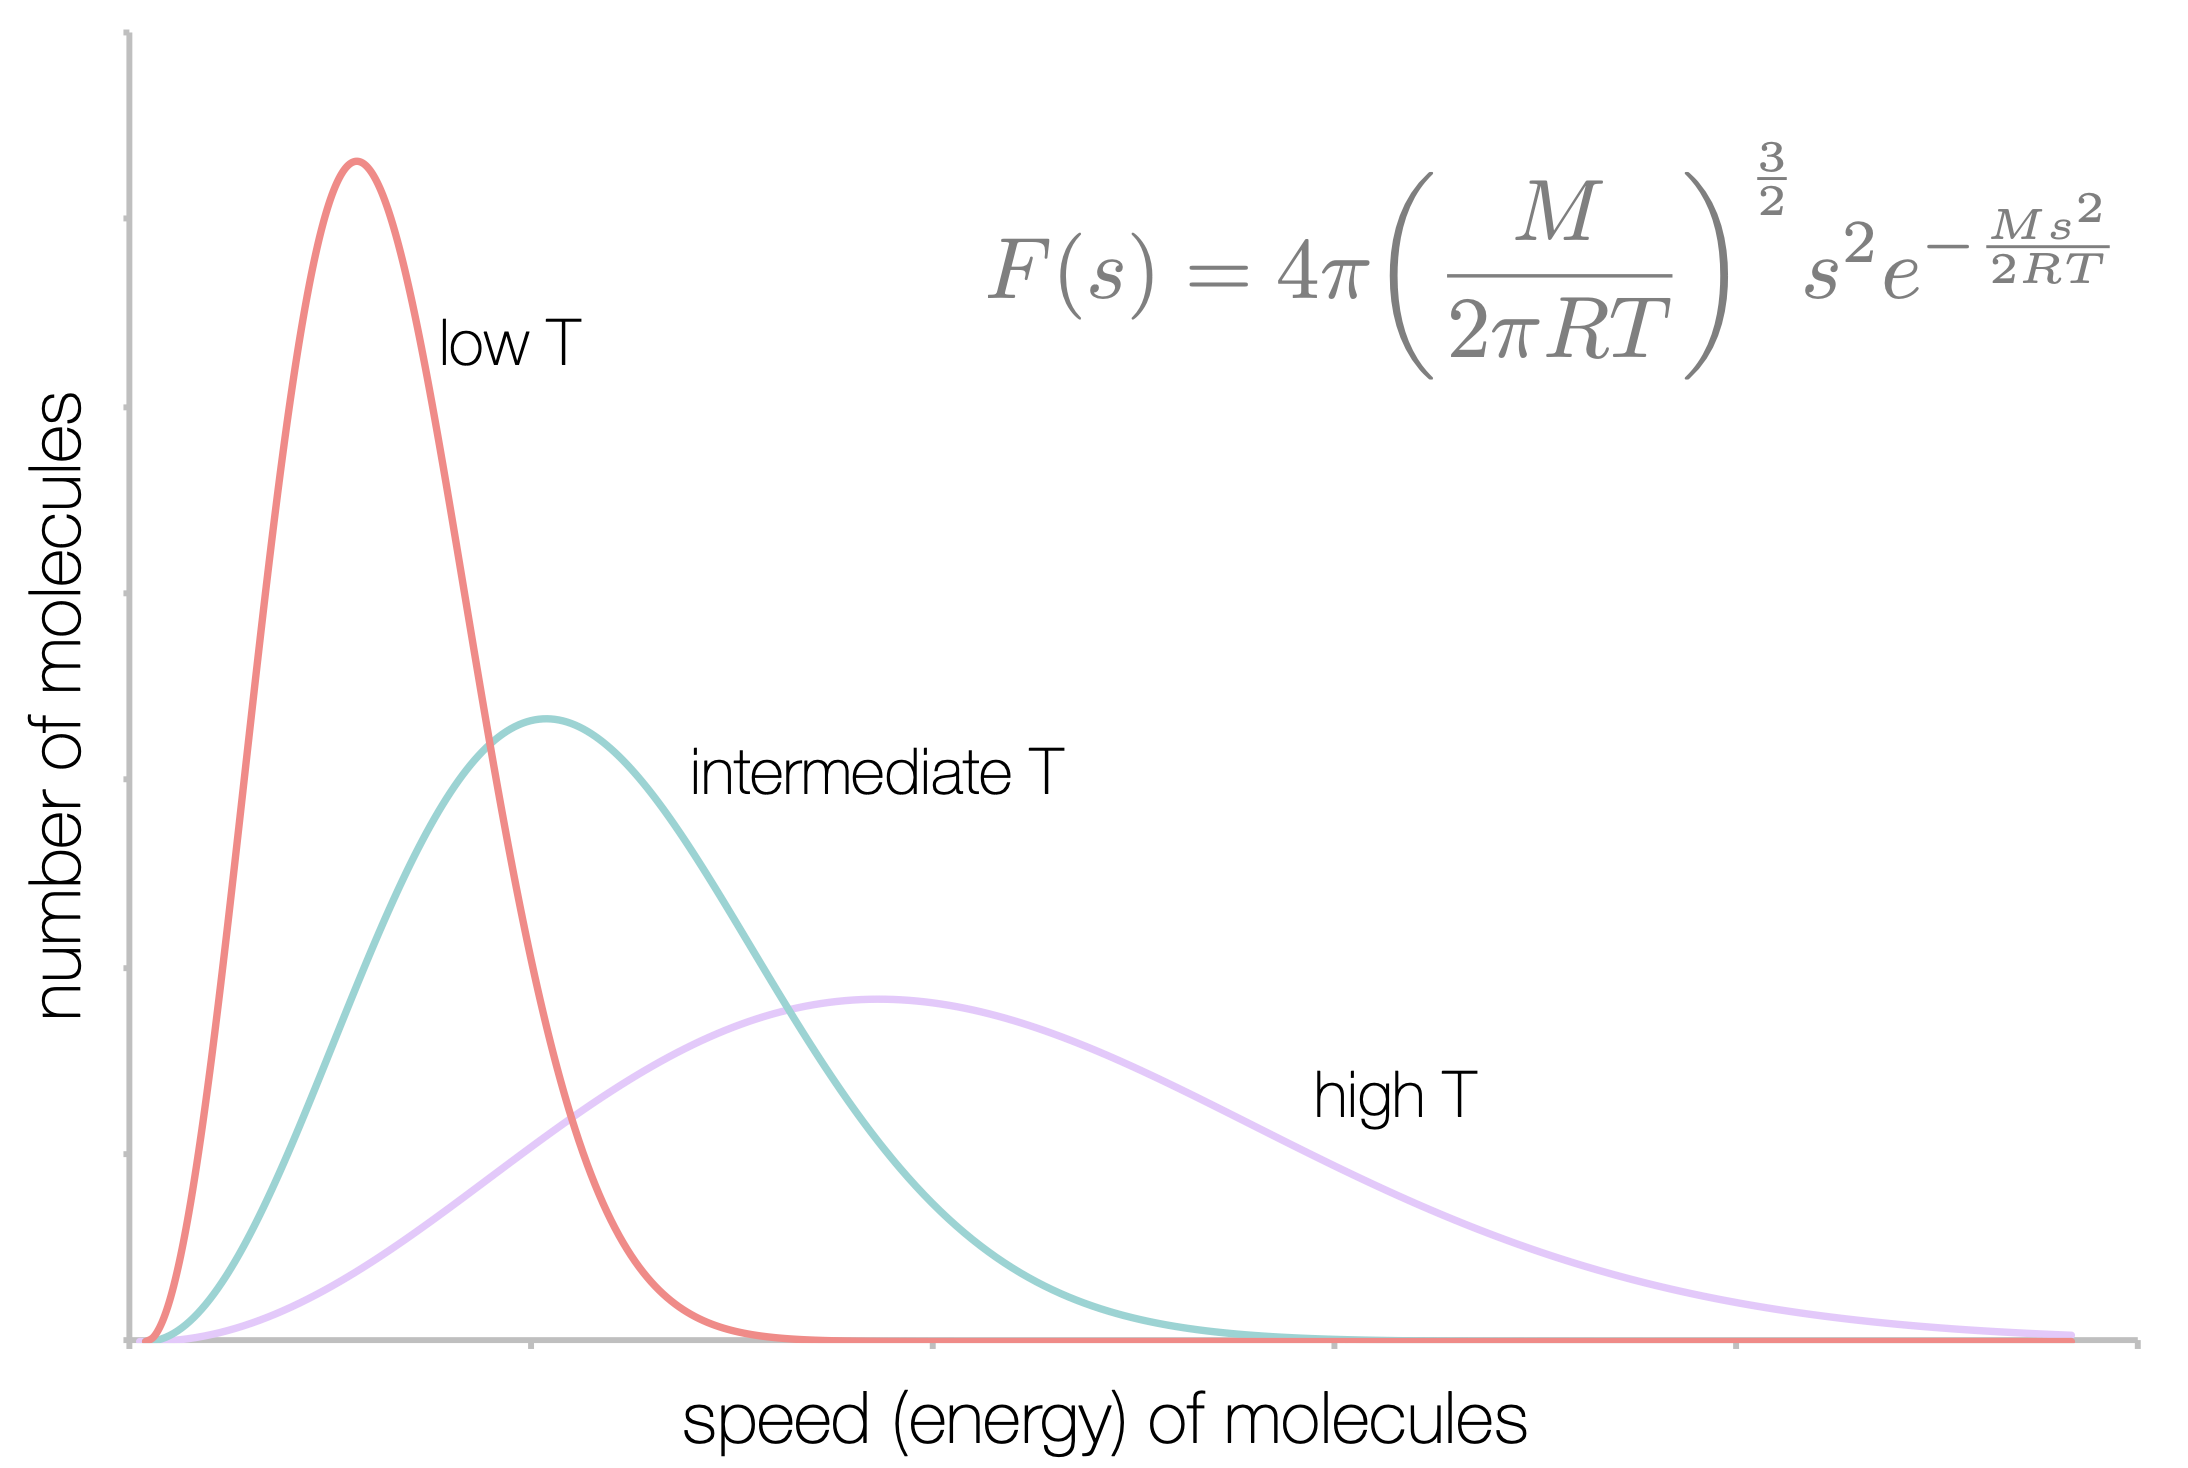
\includegraphics[width=0.8\linewidth]{images/boltzmann} 

}

\caption{The distribution of speeds of a gas depends only upon temperature and molecular mass. At low temperatures the mean speeds of particles are lower than those at high temperatures.}\label{fig:boltzmann}
\end{figure}

Therefore there is fundamental link between `speed' and temperature. In Section \ref{sec:classicalstat} you were introduced to the concept of energy levels in molecules. If you recall all energy levels are quantised, and translational energy levels have the closest spacing (figure \ref{fig:energylevels}). The faster a molecule moves the higher the translational energy level it occupies.

\begin{figure}

{\centering 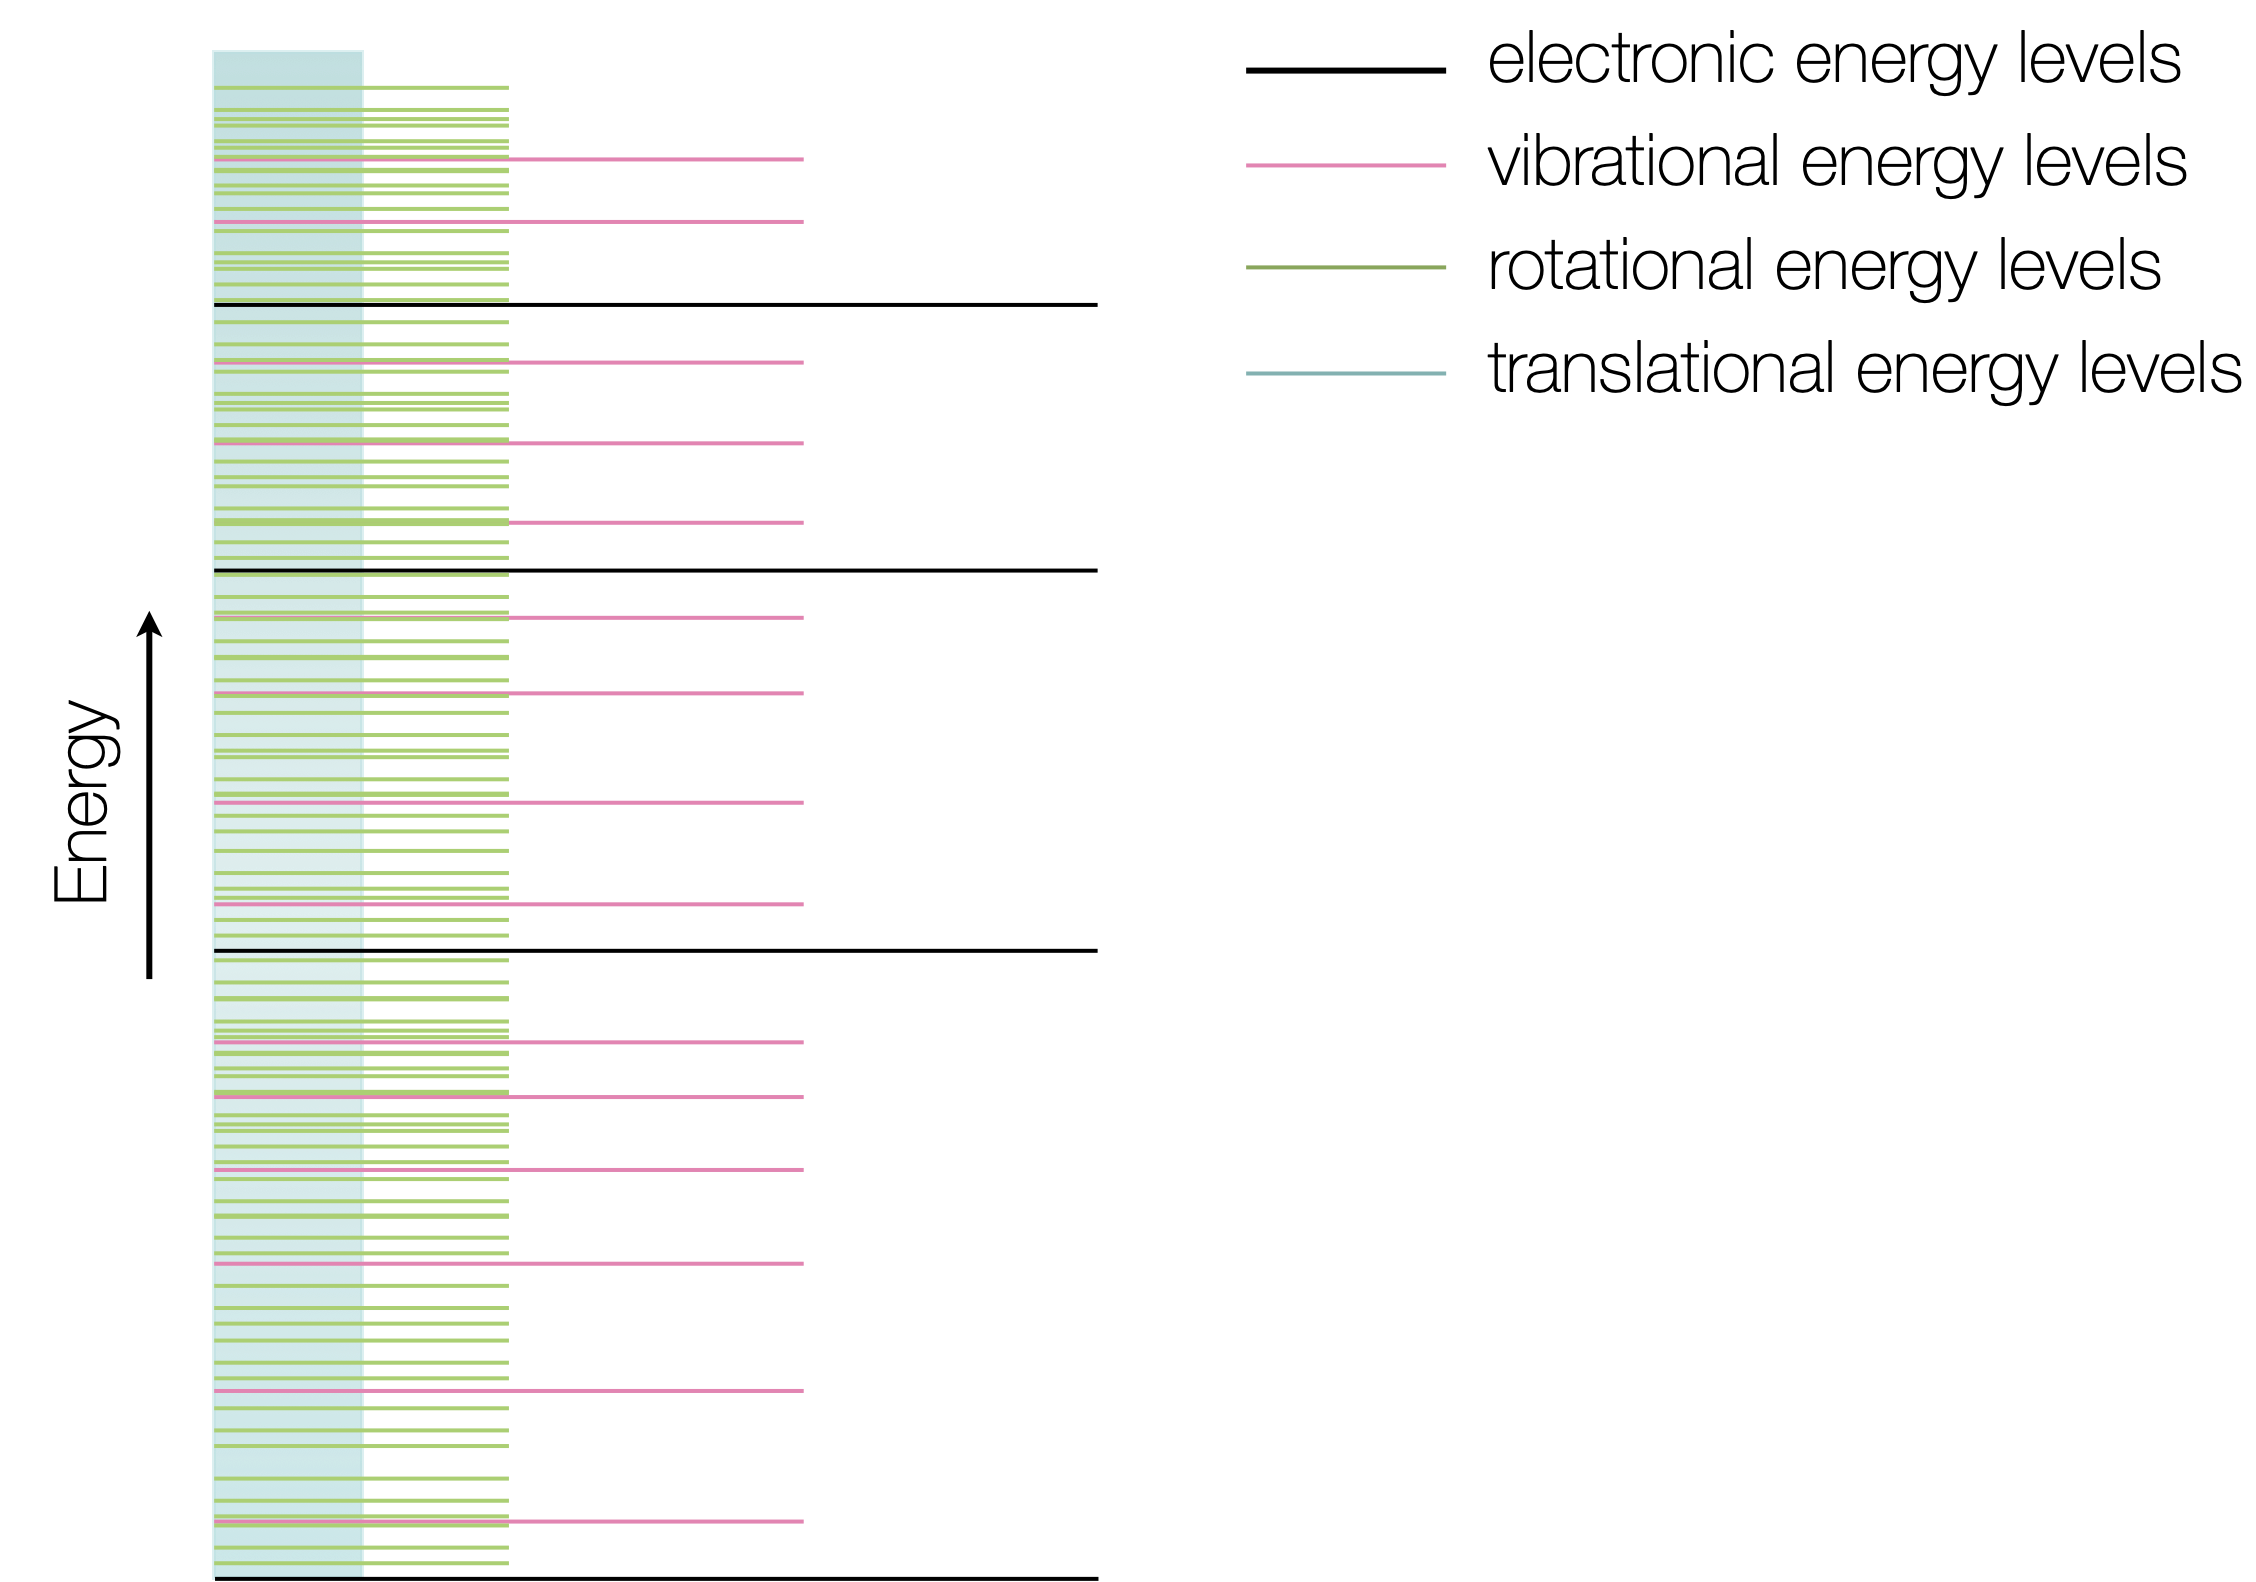
\includegraphics[width=0.8\linewidth]{images/energylevels} 

}

\caption{The energy levels within molecules have different gaps between levels, translational levels are very closely spaced, rotational energy levels have the next closest spacing, vibrational levels are higher in energy still, finally electronic levels have the largest energy gaps.}\label{fig:energylevels}
\end{figure}

The relative populations of these energy levels is given by the Maxwell-Boltzmann equation:

\begin{equation}
\frac{N_i}{N_j}=\frac{g_i}{g_j} \textrm{e}^{-\frac{\Delta E}{k_B T}}
\label{eq:maxwell}
\end{equation}

Looking at equation \eqref{eq:maxwell} we can see that the relative population of energy levels depends upon ΔE, the energy gap between them. This means that the closely spaced translational energy levels are well populated and the particles have a range of speeds associated with this.

At very low temperatures only translational levels are populated, but as the temperature increases and the energy is distributed over more levels rotational levels are then populated, then finally vibrational, at room temperature only there is only a negligible probability of vibrational energy levels being populated.

\begin{figure}

{\centering 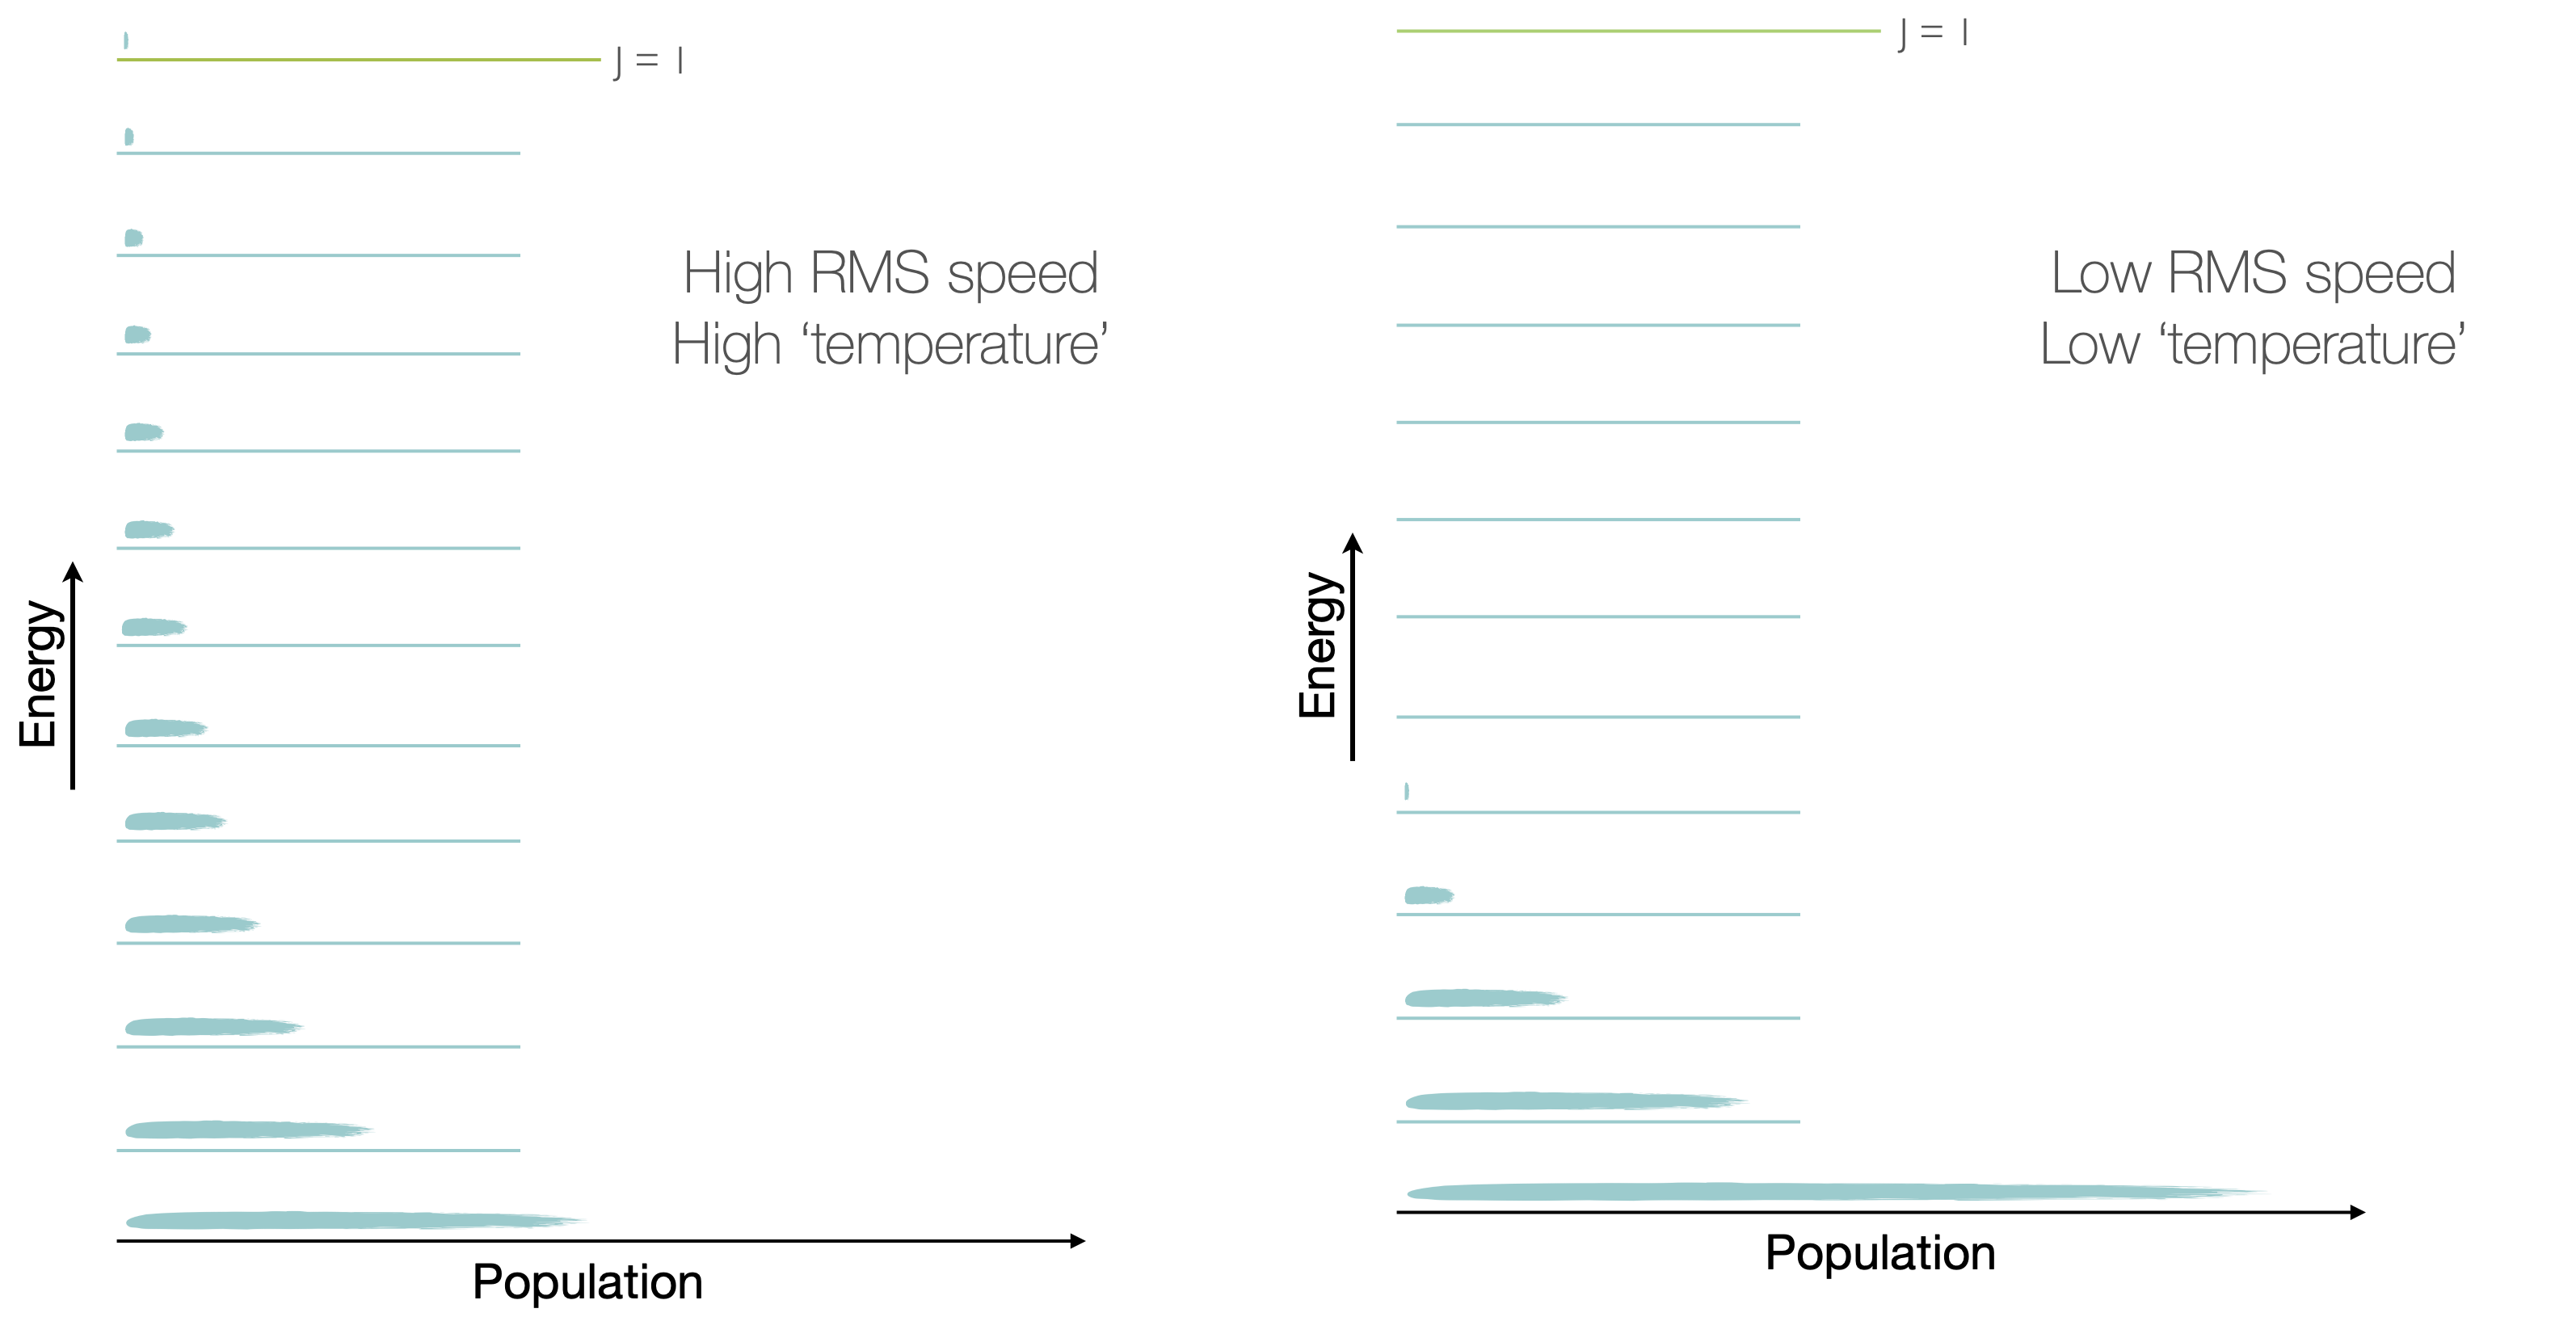
\includegraphics[width=0.8\linewidth]{images/approachingzero} 

}

\caption{As the temperature is decreased the probability of finding particles in the ground translational state increases. At absolute zero all molecules will be in the ground translational state. }\label{fig:approachingzero}
\end{figure}

Therefore temperature is a measure of the population of energy levels within a molecule.

\hypertarget{internal-energy-u}{%
\section{Internal energy, U}\label{internal-energy-u}}

Internal energy is a state function (equation \eqref{eq:internal}), which describes the `total internal energy' of a system. We are already aware that there is thermal energy within the system from the population of the energy levels as described in figure \ref{fig:energylevels}. However internal energy also accounts for the `potential energy' from the inter- and intra- molecular interactions between particles in the system (figure \ref{fig:internalenergy}).

\begin{figure}

{\centering 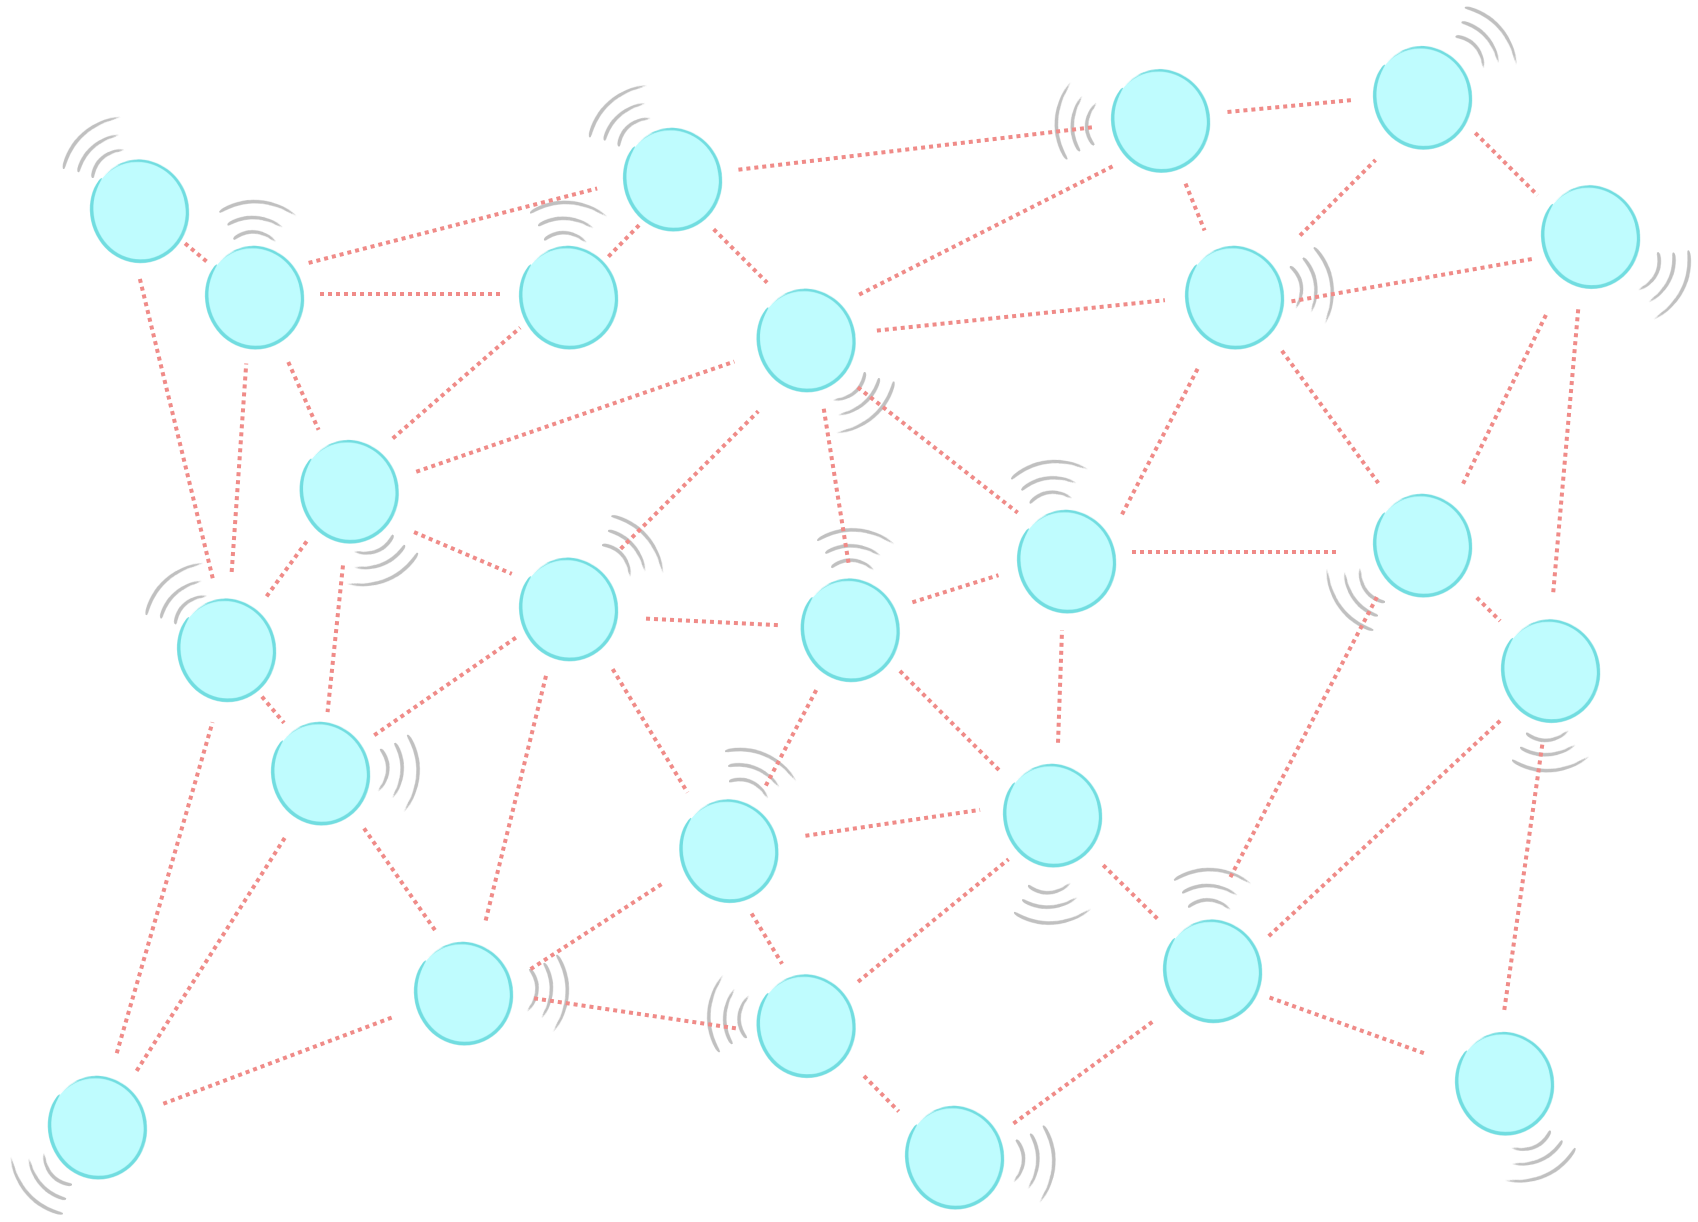
\includegraphics[width=0.8\linewidth]{images/internalenergy} 

}

\caption{The internal energy of a system is the sum of the kinetic and potential energies of the particles in the system.}\label{fig:internalenergy}
\end{figure}

Since internal energy is a state function the change in internal energy in a process is given by the difference in internal energy of the final and initial states (equation \eqref{eq:internal}).

\begin{equation}
\Delta U = U_\textrm{f} - U_\textrm{i}
\label{eq:internal}
\end{equation}

\hypertarget{degrees-of-freedom}{%
\subsection{Degrees of Freedom}\label{degrees-of-freedom}}

NOTE - I've also added this to the week1 part1 so this section is duplicated.

Perhaps unsurprisingly the structure of molecules is an important concept when we consider thermodynamics from the molecule up perspective, but perhaps surprisingly classical thermodynamics does not care at all the structure of the molecules in the system we are considering.

\begin{figure}

{\centering 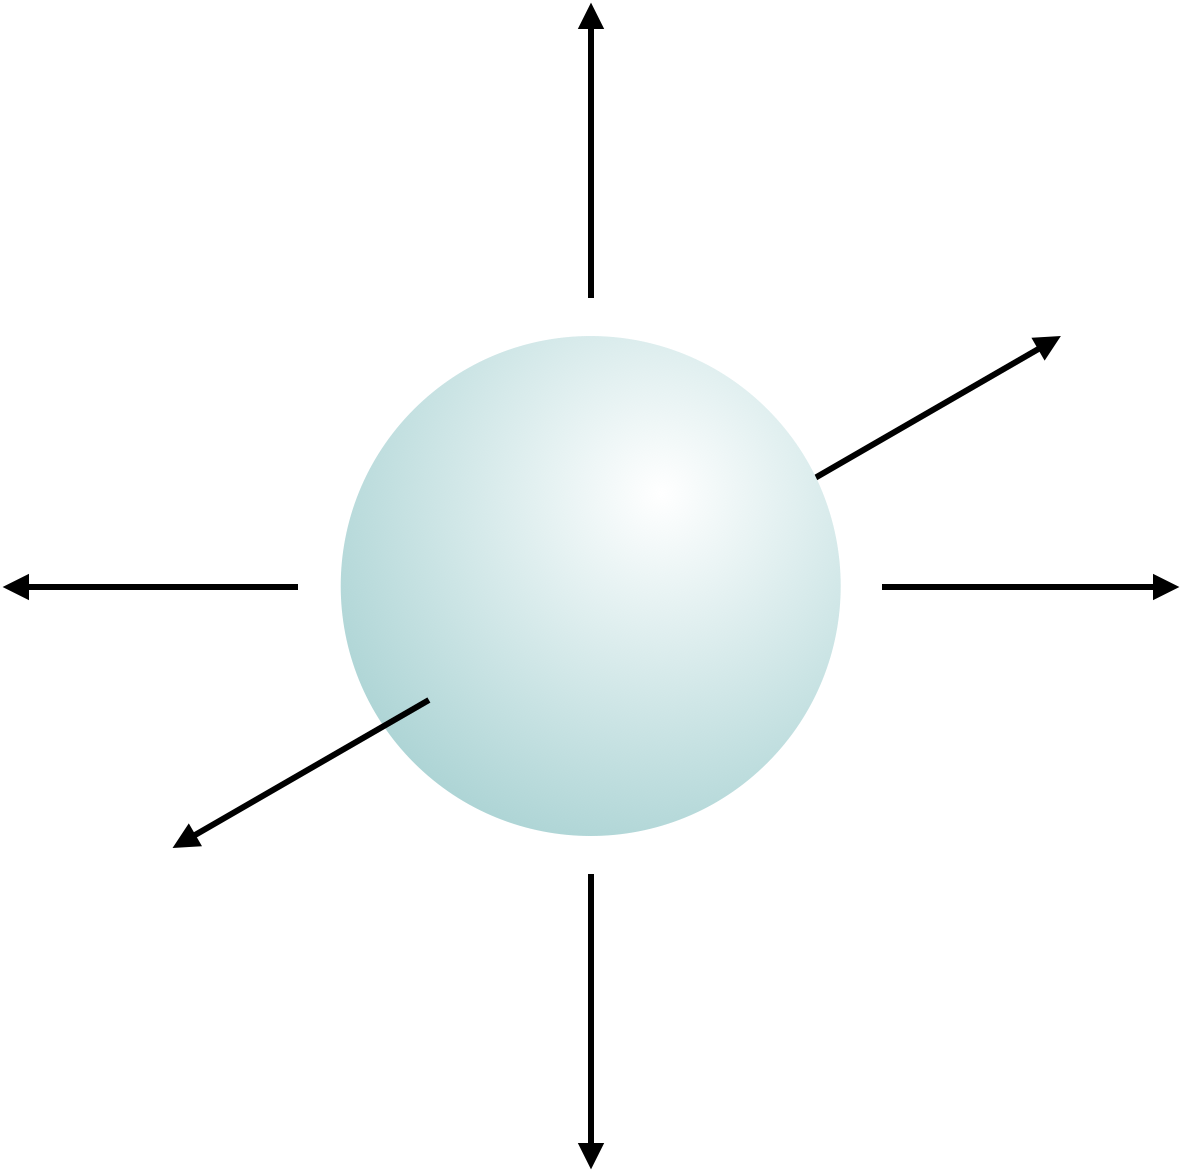
\includegraphics[width=0.5\linewidth]{images/atomdegrees} 

}

\caption{Every atom has three degrees of freedom, these are movement along the x, y and z axis.}\label{fig:atomdegrees1}
\end{figure}

When atoms combine to form moleucules the total number of degrees of freedom must be conserved, and so new types of degrees of freedom are introduced, namely molecular rotations and molecular vibrations (figure \ref{fig:typesdegree1}, and equations \eqref{eq:lineardof1} and \eqref{eq:nonlineardof1}).

\begin{figure}

{\centering 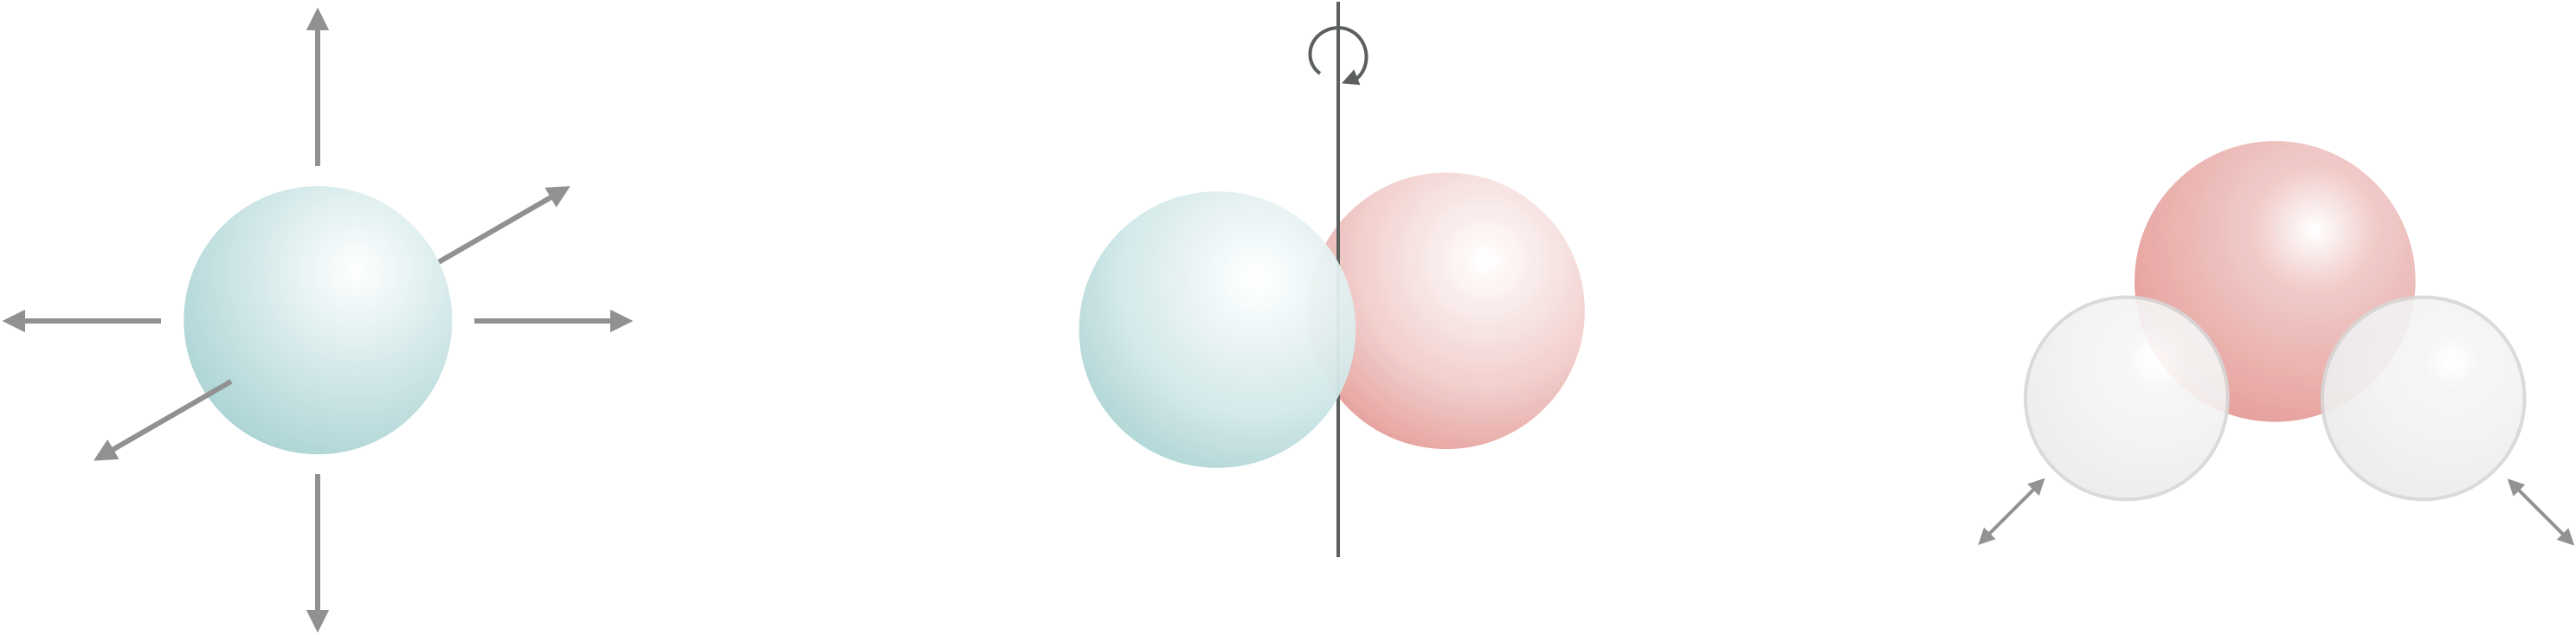
\includegraphics[width=0.8\linewidth]{images/typesdegree} 

}

\caption{Translations, molecular rotations and molecular vibrations are all degrees of freedom.}\label{fig:typesdegree1}
\end{figure}

For linear molecules there are three translational degrees of freedom, two rotational degrees of freedom (figure \ref{fig:linear1}) and the number of vibrational degrees of freedom is given by equation \eqref{eq:lineardof1}, where N is the total number of atoms in the molecule:

\begin{equation}
x = 3N-5
\label{eq:lineardof1}
\end{equation}

\begin{figure}

{\centering 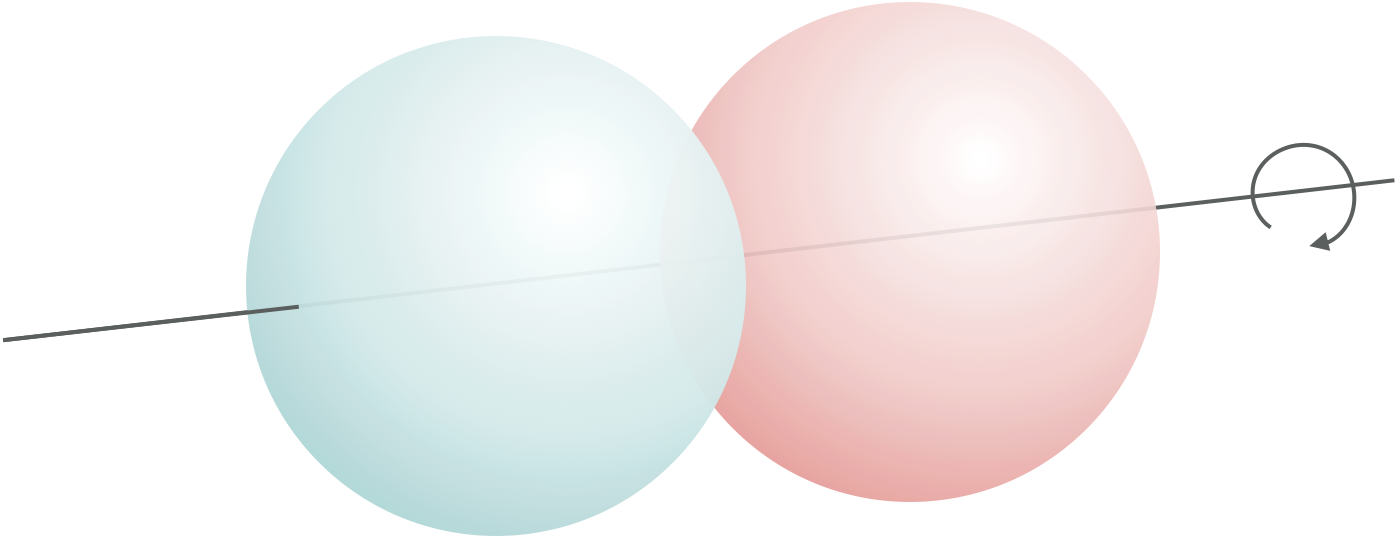
\includegraphics[width=0.8\linewidth]{images/linear} 

}

\caption{In linear molecules there are only two rotational degrees of freedom as rotaion around the z-axis (the long axis of the molecule) are equivalent and therefore dont contribute to the degrees of freedom.}\label{fig:linear1}
\end{figure}

For non-linear molecules there are three translational degrees of freedom, three rotational degrees of freedom and the number of vibrational degrees of freedom is given by equation \eqref{eq:nonlineardof1}, again where N is the total number of atoms in the molecule:

\begin{equation}
x = 3N-6
\label{eq:nonlineardof1}
\end{equation}

\hypertarget{subsec:equipartition}{%
\subsection{Equipartition theory}\label{subsec:equipartition}}

\emph{Some of the material covered in this video relates to heat capacities which we will study in more detail later in the course.}

Equipartition theory is quite involved, and I am not going to explain any of the actual theory or derivation in this course, instead we are going to just use the results of this theory.

These results from statistical thermodynamic calculation, are verified by emperical observations which is proof of the power of Boltzmann's theories.

Equipartition theory says that for an ideal gas each degree of freedom contributes \(\frac{RT}{2}\) to the molar internal energy, and so for monatomic gases, such as helium and neon the internal energy , U is \(\frac{3RT}{2}\). However for a diatomic gas with 6 degrees of freedom (3 translational, 2 rotational and 1 vibrational) the internal energy of the ideal gas is predicted to be \(3RT\).

However, we have already seen that the energy spacing between different types of energy level differs, and so only \emph{active} degrees of freedom contribute to the internal energy. Consequently because there are large energy gaps for vibrational energy levels the excited states of these energy levels are rarely occupied and so they do not contribute towards the total internal energy of the system.

\hypertarget{first-law-of-thermodynamics}{%
\section{First Law of Thermodynamics}\label{first-law-of-thermodynamics}}

There are a number of variations on the statements of the first law of thermodynamics, but ultimately they are all saying the same thing. The variations come from different definitions referring to different types of thermodynamic system (Section \ref{sec:typesofsystem}).

The first statement of the first law of thermodynamics is the most fundamental:

\emph{`the internal energy of an isolated system is constant'}

This should be fairly obvious, if my system is isolated there can be no exchange of matter or energy and so the internal energy can't change.

A second version of first law refers to a closed system, one where there can be no exchange of matter, but energy may be exchanged in the form of either heat or work. Mathematically this statement is (\eqref{eq:firstlaw}):

\begin{equation}
\Delta U = q + w
\label{eq:firstlaw}
\end{equation}

where \(q\) is the energy exchanged in the form of heat and \(w\) the energy exchanged in the form of work.

\hypertarget{questions}{%
\section{Questions}\label{questions}}

1. Determine the number of degrees of freedom in each of the following molecules, and consequently predict the molar internal energy at 25 ºC.

\begin{enumerate}
\def\labelenumi{\alph{enumi}.}
\tightlist
\item
  molecular nitrogen, N\textsubscript{2}
\item
  ozone, O\textsubscript{3}
\item
  acetylene HCCH
\end{enumerate}

\begin{enumerate}
\def\labelenumi{\arabic{enumi}.}
\setcounter{enumi}{1}
\item
  Why can't you use equipartition theory to determine the internal energy of ethanol at room temperature?
\item
  If a system looses 250 J of energy from loss of heat, and 600 J of energy is added to the sytem in the form of work what is the change in internal enery of the system, and the universe?
\item
  How does changing the spacing of energy levels change the distribution of population of energy levels in a system?
\end{enumerate}

\hypertarget{answers}{%
\section{Answers}\label{answers}}

\begin{enumerate}
\def\labelenumi{\arabic{enumi}.}
\item
  \begin{itemize}
  \item
  \end{itemize}
\end{enumerate}

\begin{enumerate}
\def\labelenumi{\alph{enumi}.}
\tightlist
\item
  6.194 kJ mol\textsuperscript{−1}
\item
  7.433 kJ mol\textsuperscript{−1}
\item
  6.194 kJ mol\textsuperscript{−1}
\end{enumerate}

\begin{enumerate}
\def\labelenumi{\arabic{enumi}.}
\setcounter{enumi}{1}
\item
  It's a liquid at room temperature, equipartition theory tells us about ideal gases.
\item
  \(\Delta U_{system}=\) +350 J, \$\Delta U\_\{universe\}=\$0J
\item
  It shouldn't they will respace, so if the population of levels is higher when the space is bigger, but you are just distributing the energy differently.
\end{enumerate}

\hypertarget{ch:Part3}{%
\chapter{Week 2 - Part 1}\label{ch:Part3}}

Previously we have been introduced to the concepts of temperature and internal energy, two fundamental concepts in thermodynamics, and we finished by introducing the first law of thermodynamics, and introducing the terms `heat' and `work'. In this part we learn what heat and work are thermodynamically, and extend our idea of state functions to bring the well known concept of Hess' Law to this course.

The unit of energy is joule, this is named after one of the pioneers of thermodynamics.

\emph{The following video has been added for some context to the material, it is not core to the course and the material in it is not examinable.}

\hypertarget{sec:work}{%
\section{Work, w}\label{sec:work}}

In thermodynamics the term `work' describes a mode of transfer of energy between the system and surroundings, this transfer of energy achieves a uniform motion. Work is sometimes considered to be useful energy because this uniform motion may be used to move a piston, lift a weight in a gravitational field or power a phone.

\begin{figure}

{\centering 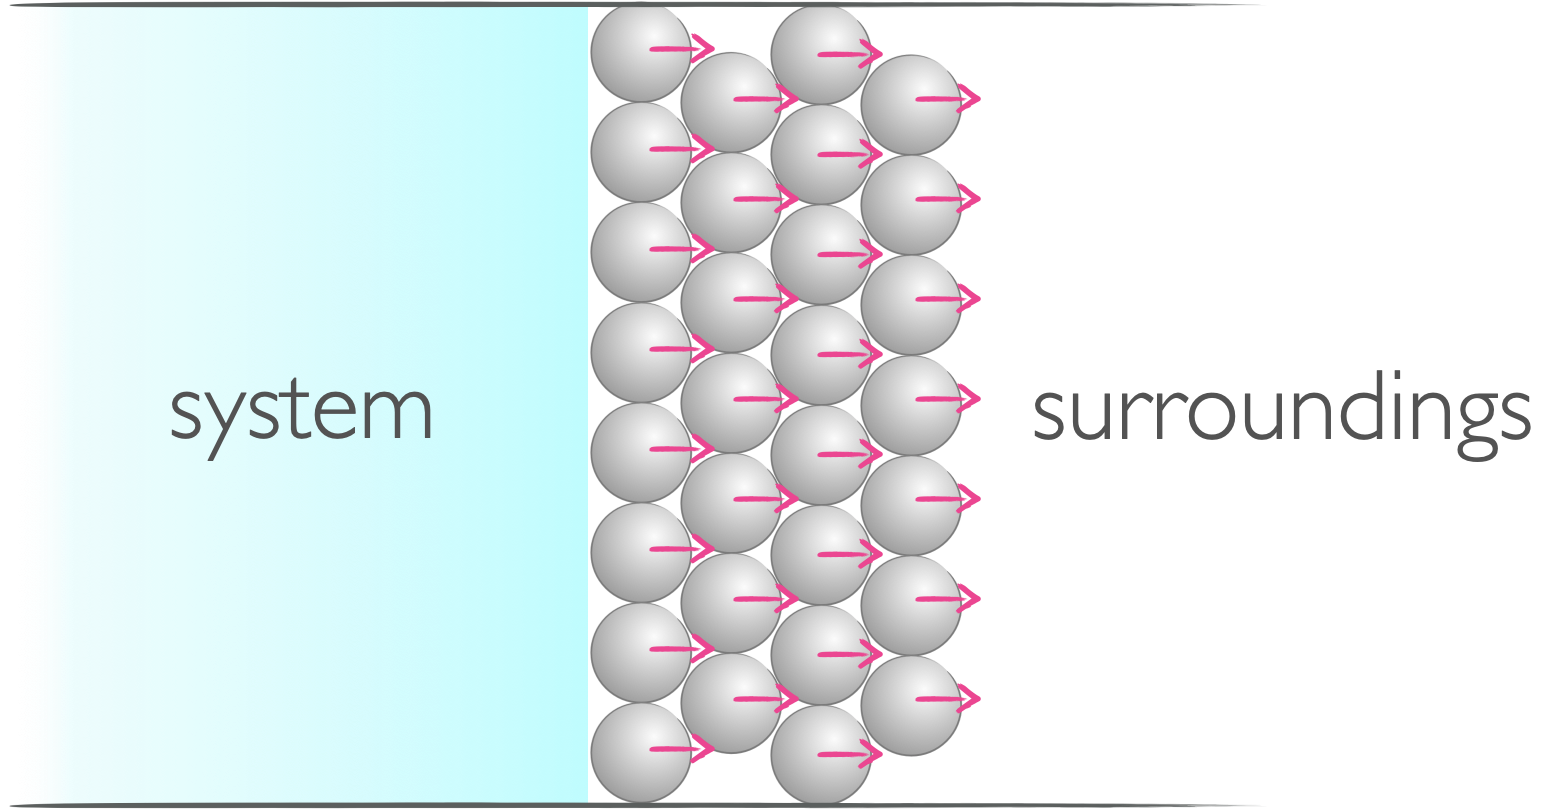
\includegraphics[width=0.5\linewidth]{images/work} 

}

\caption{When energy is transfered in the form of work there is a uniform change in the system or surroundings.}\label{fig:work}
\end{figure}

If we consider the expansion of a gas in a piston against a constant external pressure the gas will expand until the pressure inside and outside of the piston are the same (figure \ref{fig:irrevexpansion}). The work done in this process is given by equation \eqref{eq:irrevexpansion}, and shown as the shaded area in figure \ref{fig:irrevexpansion}.

\begin{figure}

{\centering 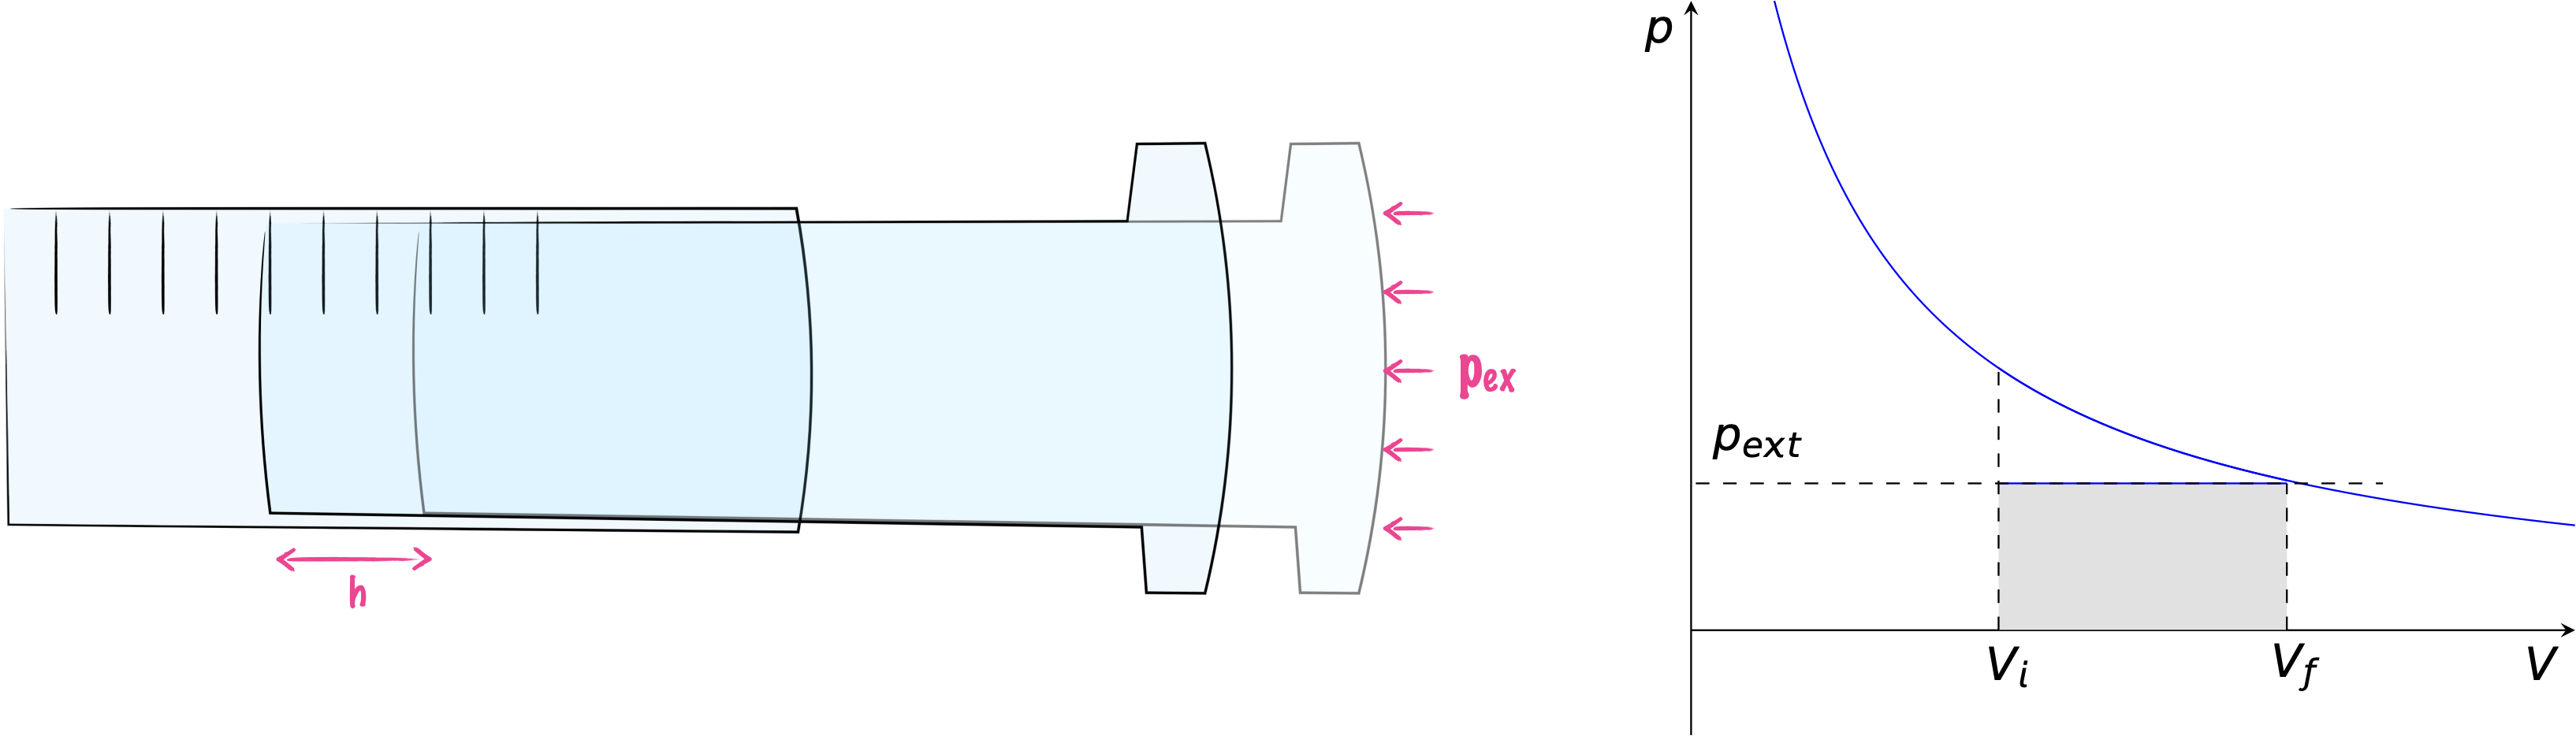
\includegraphics[width=1\linewidth]{images/irrevexpansion} 

}

\caption{If a gas expands against a constant external pressure the expansion will continue until the pressure inside and out of the piston is the same.}\label{fig:irrevexpansion}
\end{figure}

\begin{equation}
w=-p_{\textrm{ex}}\Delta V
\label{eq:irrevexpansion}
\end{equation}

The work done, is negative because if the system does work on the surroundings energy is transferred from the system to the surroundings and the internal energy of the system falls.

You can check the units of this process to help verify this statement, pressure has the units pascal, Pa, which in SI base units is kg m\textsuperscript{−1} s\textsuperscript{−2} and volume of course m\textsuperscript{3}. The units of work are joules, J, which in SI base units is kg m\textsuperscript{2} s\textsuperscript{−2}.

If we instead consider the hypothetical thermodynamically reversible process where the system and surroundings are in equilibrium all through the expansion, this tells us the maximum possible work which can be achieved from a system.

\begin{figure}

{\centering 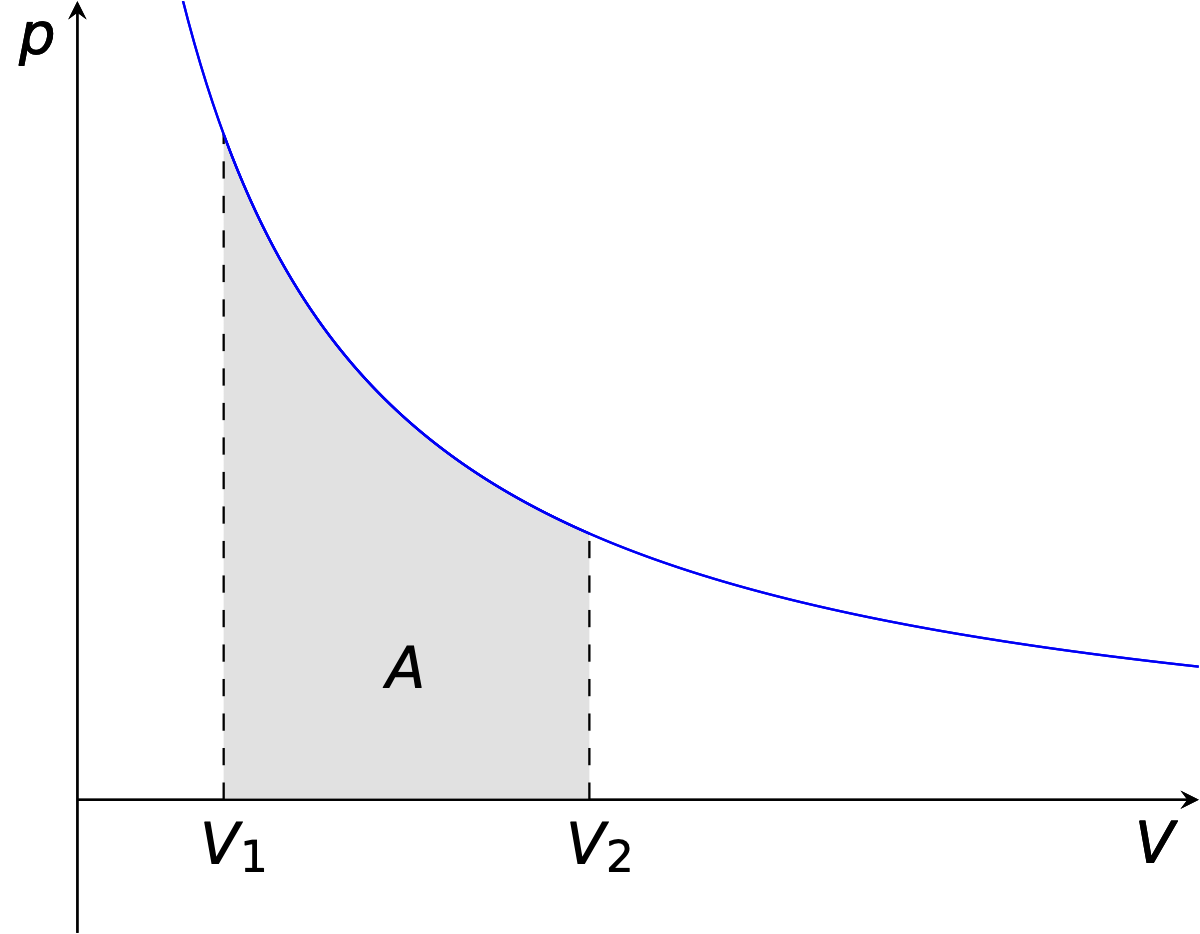
\includegraphics[width=0.5\linewidth]{images/revexpansion} 

}

\caption{If a gas expands and the pressure inside and out are only ever infitessimal difference between the pressure of system and surroundings this is called a reversible expansion and the maximum possible amount of work can be achieved.}\label{fig:revexpansion}
\end{figure}

In the case of a reversible expansion the work done by the system in an expansion is given in equation \eqref{eq:revexpansion}, this expression may be derived from integrating the area under the pV curve in figure \ref{fig:revexpansion}.

\begin{equation}
w=-n\textrm{R}T \ln {\frac{V_\textrm{f}}{V_\textrm{i}}}
\label{eq:revexpansion}
\end{equation}

For the same increase in volume at the temperature of the system increases then the work needed in a reversible expansion also increases.

There are many types of work, but they may all be modeled by expansion work. Other types of work include things like surgace expansion, extension of a spring or electrical work.

\hypertarget{sec:heat}{%
\section{Heat, q}\label{sec:heat}}

If you recall the definition of a closed system (section \ref{subsec:closed}), we introduced the concept of energy being able to be exchanged in the form of heat through a diathermic wall, this is just a boundary through which energy in the form of heat may be transferred.

Heat is defined as a mode of transfer of energy that achieves a random motion in the surroundings.

\begin{figure}

{\centering 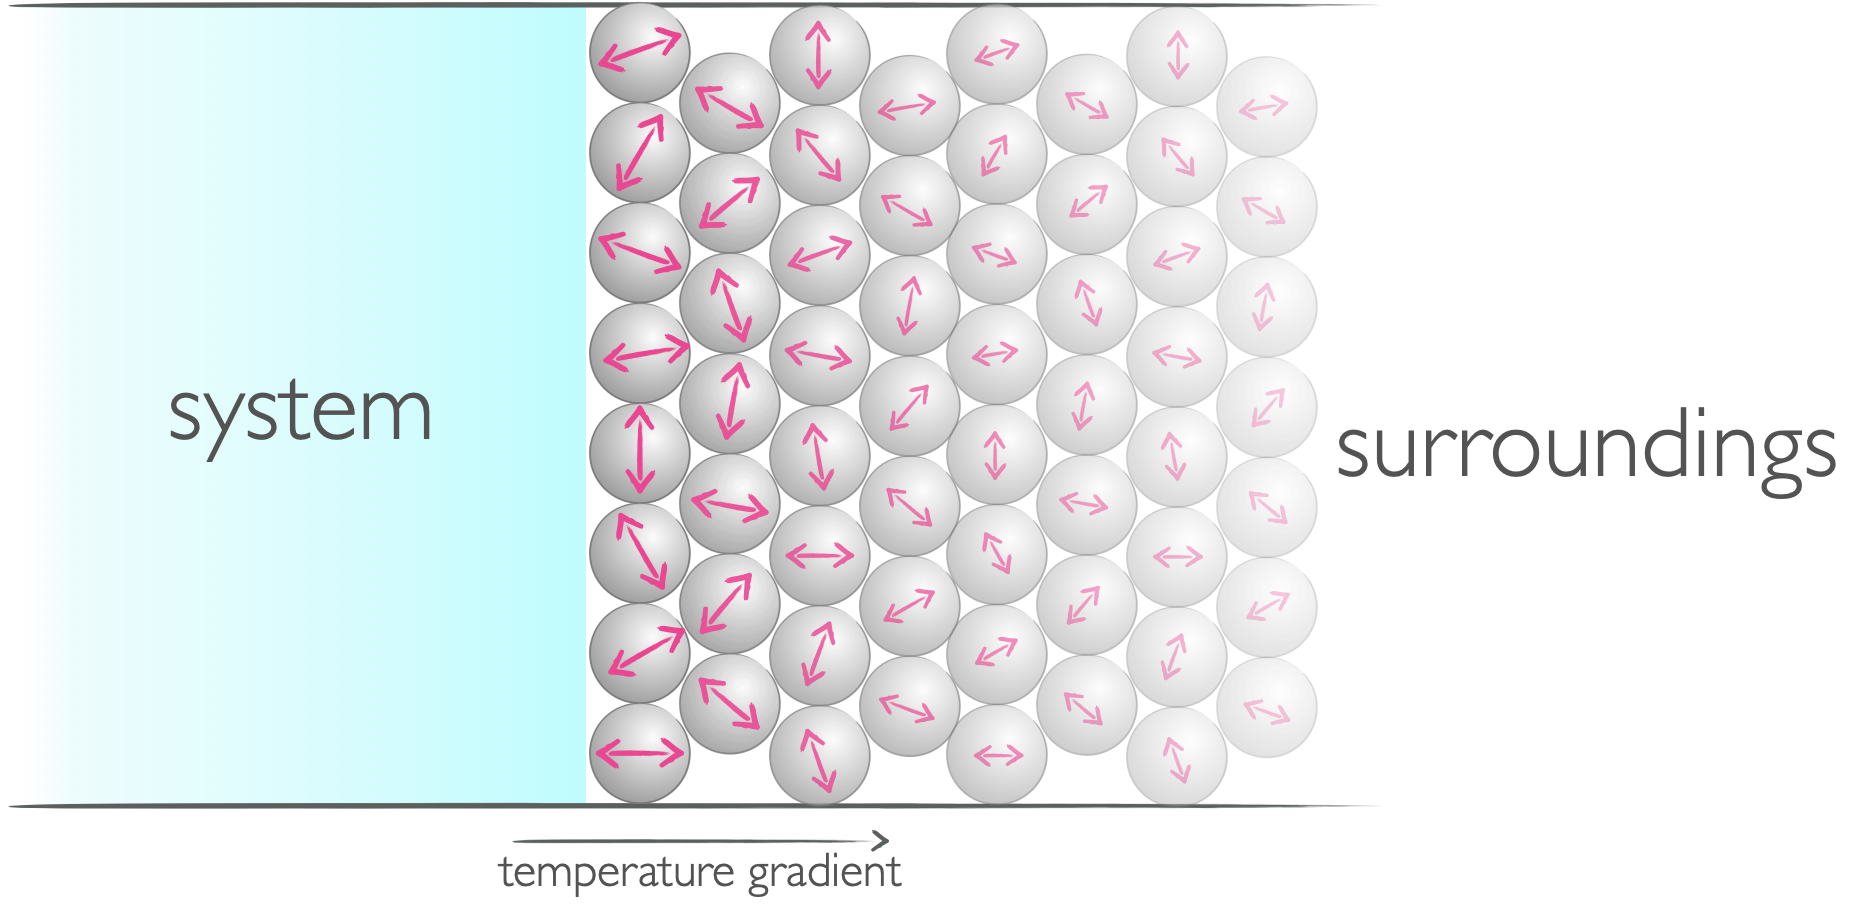
\includegraphics[width=0.5\linewidth]{images/heat} 

}

\caption{When energy is transfered in the form of heat it induces a random motion in the system or surroundings.}\label{fig:heat}
\end{figure}

\begin{itemize}
\item
  When a reaction is exothermic energy in the form of heat is transferred from the system to the surroundings and the internal energy of the system falls (q = -ve).
\item
  When a reaction is endothermic energy in the form of heat is transferred from the surroundings to the system and the internal energy of the system increases (q = +ve).
\end{itemize}

\hypertarget{isothermal-reversible-expansion}{%
\subsection{Isothermal reversible expansion}\label{isothermal-reversible-expansion}}

If a gas is allowed to expand and no heat is transferred then the work done by the system allows the temperature of the system to fall.

\begin{figure}

{\centering 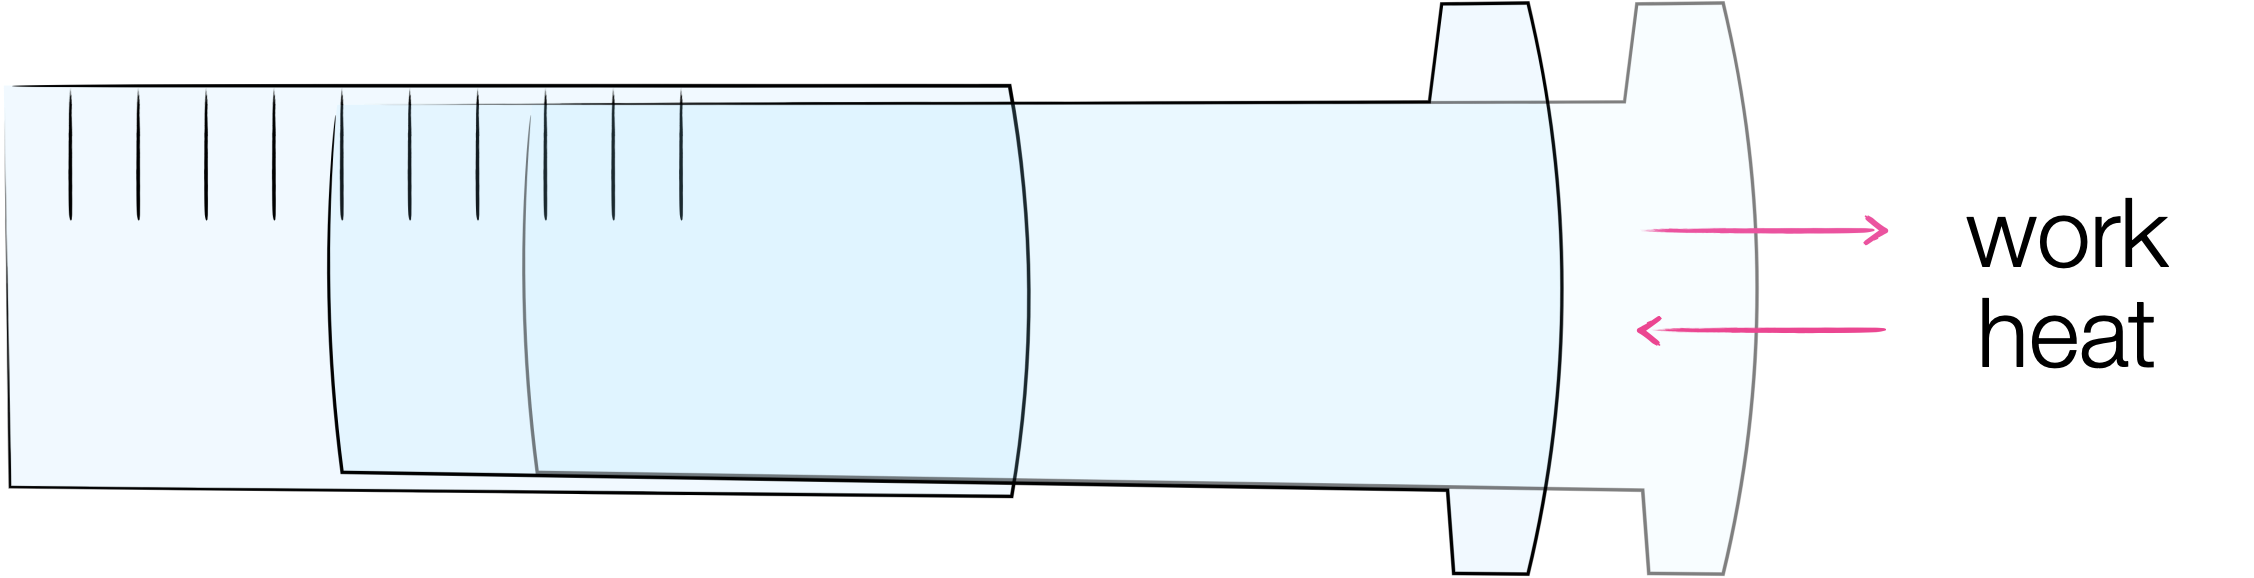
\includegraphics[width=0.5\linewidth]{images/isothermalexpansion} 

}

\caption{In the case of an isothermal reversible expansion the work done by the system and the heat transferred to the system exactly balance.}\label{fig:isothermalexpansion}
\end{figure}

There is a special case where we can consider the expansion of a gas but energy is transferred from the surroundings to the system in the form of heat. In this isothermal reversible expansion the work done by the system is exactly equal an opposite to the heat transferred to the system, and so the net change in internal energy is zero.

Therefore, by applying this to equation \eqref{eq:revexpansion}, we can see for an isothermal reversible expansion:

\begin{equation}
q=n\textrm{R}T \ln {\frac{V_\textrm{f}}{V_\textrm{i}}}
\label{eq:isothermalexpansion}
\end{equation}

This is just an example of the first law of thermodynamics in action.

\hypertarget{enthalpy-h}{%
\section{Enthalpy, H}\label{enthalpy-h}}

The enthalpy of a system is given by:

\begin{equation}
H = U+pV
\label{eq:enthalpy}
\end{equation}

at constant pressure the enthalpy change of a system is given by:

\begin{equation}
\Delta H = \Delta U + p\Delta V
\label{eq:enthalpychange}
\end{equation}

Fundamentally enthalpy is a way of keeping track of internal energy when we are working in systems which are at constant pressure, systems which are allowed to do expansion work against the atmosphere.

If we take both our original definitions of enthalpy and internal energy we can bring enthalpy back to a concept I am sure you are all familiar. That being heat:

\begin{equation*}
\Delta H = \Delta U + p\Delta V
\end{equation*}

and

\begin{equation*}
\Delta U = w + q
\end{equation*}

then

\begin{equation*}
\Delta H = w + q + p \Delta V
\end{equation*}

Therefore:

\begin{equation}
\Delta H_p = q
\label{eq:enthalpyconstp}
\end{equation}

Consequtnly at 25 ºC the molar enthalpy of an ideal gas is about 2.5 kJ mol\textsuperscript{−1}

\hypertarget{hesss-law}{%
\section{Hess's Law}\label{hesss-law}}

Just like internal energy, enthalpy is a state function, and the relationship between the enthalpy of a reaction is just the difference in enthalpy of the final and initial states.

Hess' law (equation \eqref{eq:enthalpystate1})is just application of the nature of enthalpy being a state function:

\begin{equation}
\Delta_r H^{\ominus} = \sum_{products}v \Delta H^{\ominus}_\textrm{X}-\sum_{reactants}v \Delta H^{\ominus}_\textrm{X}
\label{eq:enthalpystate1}
\end{equation}

If the enthalpy of reaction is positive the reaction is endothermic heat is transferred from the surroundings to the system and the temperature of the surroundings falls, if the enthalpy of reaction is negative the reaction is exothermic heat is transferred from the system to the surroundings and the temperature of surroundings increases.

\hypertarget{constant-volume-and-constant-pressure}{%
\subsection{Constant volume and constant pressure}\label{constant-volume-and-constant-pressure}}

This is just to highlight that at constant volume the system cannot expand and therefore no work can be done, consequently \(\Delta U_V = q\).

At constant pressure the work done, \(-p \Delta V\) means that the change in enthalpy (\(\Delta H = \Delta U + p \Delta V\)) is given by \(\Delta H_p=q\).

\hypertarget{questions}{%
\section{Questions}\label{questions}}

\begin{enumerate}
\def\labelenumi{\arabic{enumi}.}
\item
  When exactly one mole of an ideal gas is `heated' with 1.75 kJ of energy, it expands doing 250 J of work. What is the change in internal energy of the gas?
\item
  Suppose we have two otherwise identical calorimeters, one calorimeter of fixed volume (isochoric) and the other calorimeter of fixed pressure (isobaric). If exactly the same amount of substance was burnt in excess oxygen in each, which would record the highest temperature change in the surroundings?
\end{enumerate}

\begin{itemize}
\tightlist
\item
  it would be the same in each
\item
  the isochoric system
\item
  the isobaric system
\item
  not enough information to determine
\end{itemize}

\begin{enumerate}
\def\labelenumi{\arabic{enumi}.}
\setcounter{enumi}{2}
\item
  For a reaction conducted at constant pressure and at 20.0 ºC the change in the number of moles of gas (\(\Delta n_{gas}\)) is +2. Calculate the difference between \(\Delta H\) \& \(\Delta U\).
\item
  Calculate the standard enthalpy of formation of \(N_2 O_5\) from the following data:
\end{enumerate}

\(2 NO_{(g)} + O_{2(g)} \longrightarrow 2 NO_{2(g)}\) \(\Delta _r H^\ominus = -114.1\) kJ mol\(^{-1}\)

\(4 NO_{2(g)} + O_{2(g)} \longrightarrow 2 N_2 O_{5(g)}\) \(\Delta _r H^\ominus = -110.2\) kJ mol\(^{-1}\)

\(N_{2(g)} + O_{2(g)} \longrightarrow 2 NO_{(g)}\) \(\Delta _r H^\ominus = +180.5\) kJ mol\(^{-1}\)

\begin{enumerate}
\def\labelenumi{\arabic{enumi}.}
\setcounter{enumi}{4}
\item
  Calculate the expansion work done on the system when 9.576 g of solid ammonium chloride, NH\textsubscript{4}Cl, decomposes completely to yield gaseous ammonia, NH3 and hydrogen chloride, HCl at a temperature of 1,410 K. Treat the expansion as irreversible and the gases formed as perfect.
\item
  What is the maximum amount of work available when 1 mole of a gas doubles in volume at 25\(^\circ\)C?
\end{enumerate}

\begin{itemize}
\tightlist
\item
  How does this change with increasing temperature?
\item
  If the expansion is isothermal how much heat is added to the system?
  \#\# Answers
\end{itemize}

\begin{enumerate}
\def\labelenumi{\arabic{enumi}.}
\item
  \begin{itemize}
  \tightlist
  \item
    1.50 kJ
  \end{itemize}
\item
  not enough infomation to determine, we would need to know if the net change in gas molecules of the system is postive or negative.
\item
  \(\Delta H - \Delta U\) = +4.876 kJ
\item
  \(Δ_fH^\ominus\) = +11.3 kJ mol\textsuperscript{−1} per mole of N\textsubscript{2}O\textsubscript{5}
\item
  w = -4.198 kJ
\item
  w = −1.72 kJ, increases, q= -w = +1.72 kJ.
\end{enumerate}

\hypertarget{ch:Part4}{%
\chapter{Week 2 - Part 2}\label{ch:Part4}}

\hypertarget{heat-capacity-cx}{%
\section{\texorpdfstring{Heat capacity, C\textsubscript{X}}{Heat capacity, CX}}\label{heat-capacity-cx}}

The heat capacity of a material is the amount of energy required to raise the temperature of that material by 1 K, however there are many different versions of heat capacity, covering both entensive an intensive properties.

Perhaps more confusingly when looking at gases we have to consider whether the heat capacity of a material is at constant pressure or constant volume. This is because if we are at consant pressure the gas has to do work in expanding, and so heat capacitites at constant volume are always smaller than those at constant pressure.

Heat capacity varies with temperature, we can usually say values will be constant within about 100 K, but numerous measurements have been used to show that the heat capacity varies with temperature as follows:

\begin{figure}

{\centering 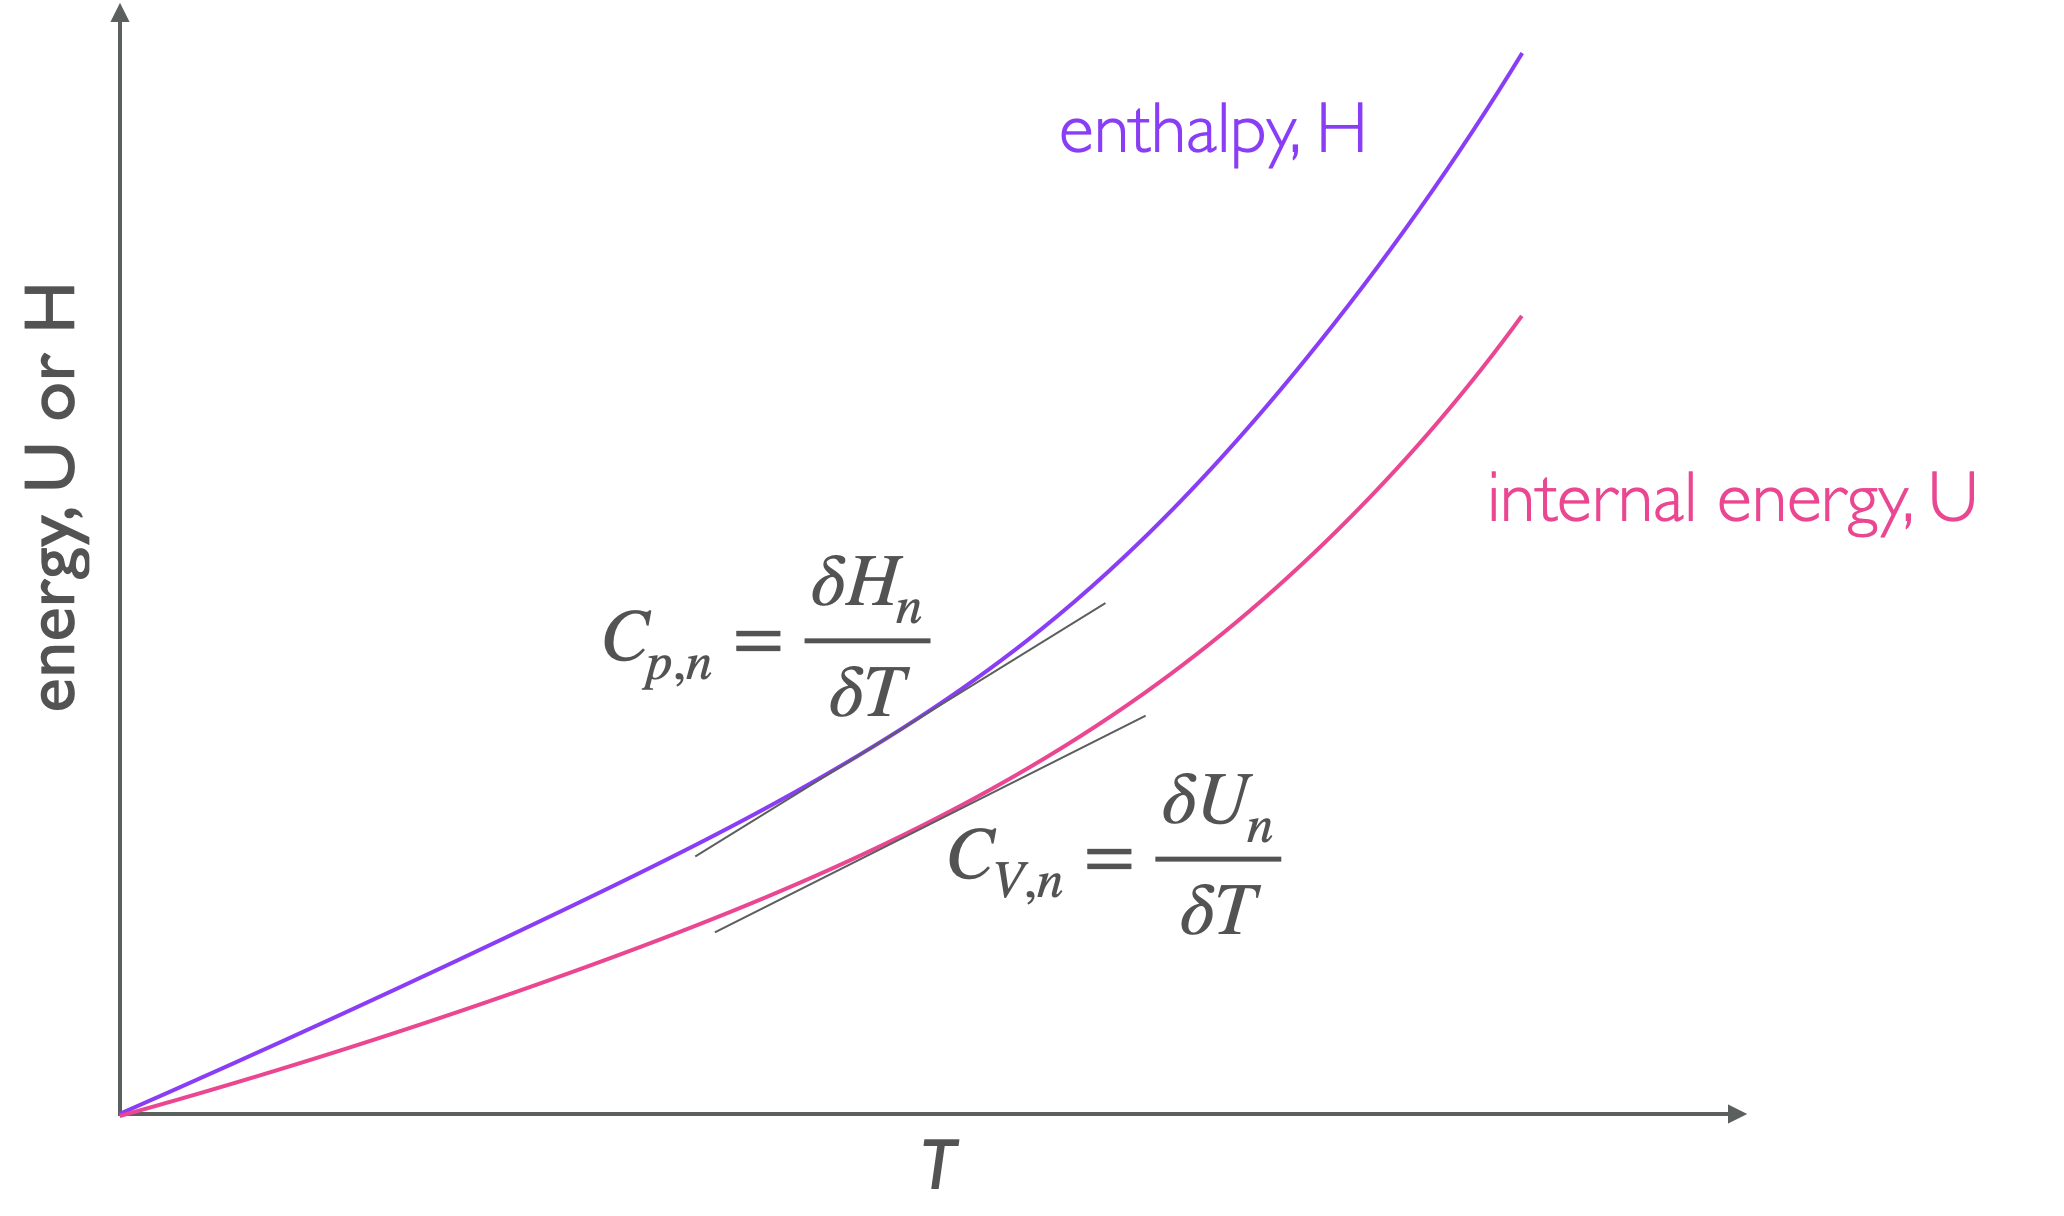
\includegraphics[width=0.7\linewidth]{images/heatcapacitypV} 

}

\caption{The heat capacity of a material is the gradient of the line on an energy verses temperature plot.}\label{fig:heatcapacitypV}
\end{figure}

\begin{equation}
C_{p,n}=\textrm{a}+\textrm{b}T+\frac{\textrm{c}}{T^2}
\label{eq:heatcapacitytemp}
\end{equation}

the constants, a, b and c are measured emperically and are known for a wide range of materials.

Previously in section @ref\{subsec:equipartition\} we have seen how equipartition theory predicts the heat capacity of ideal gases. Like the internal energy only degrees of freedom which are active contribute to heat capacity of a material, and this consideration needs to be made.

\begin{itemize}
\item
  Every translational degree of freedom contributes \(\frac{1}{2}R\) to the heat capacity
\item
  Every rotational degree of freedom contributes \(\frac{1}{2}R\) to the heat capacity
\item
  Every vibrational degree of freedom contributes \(R\) to the heat capacity
\end{itemize}

We can see the heat capacity of molecules changing as the different degrees of freedom are activated.

\begin{figure}

{\centering 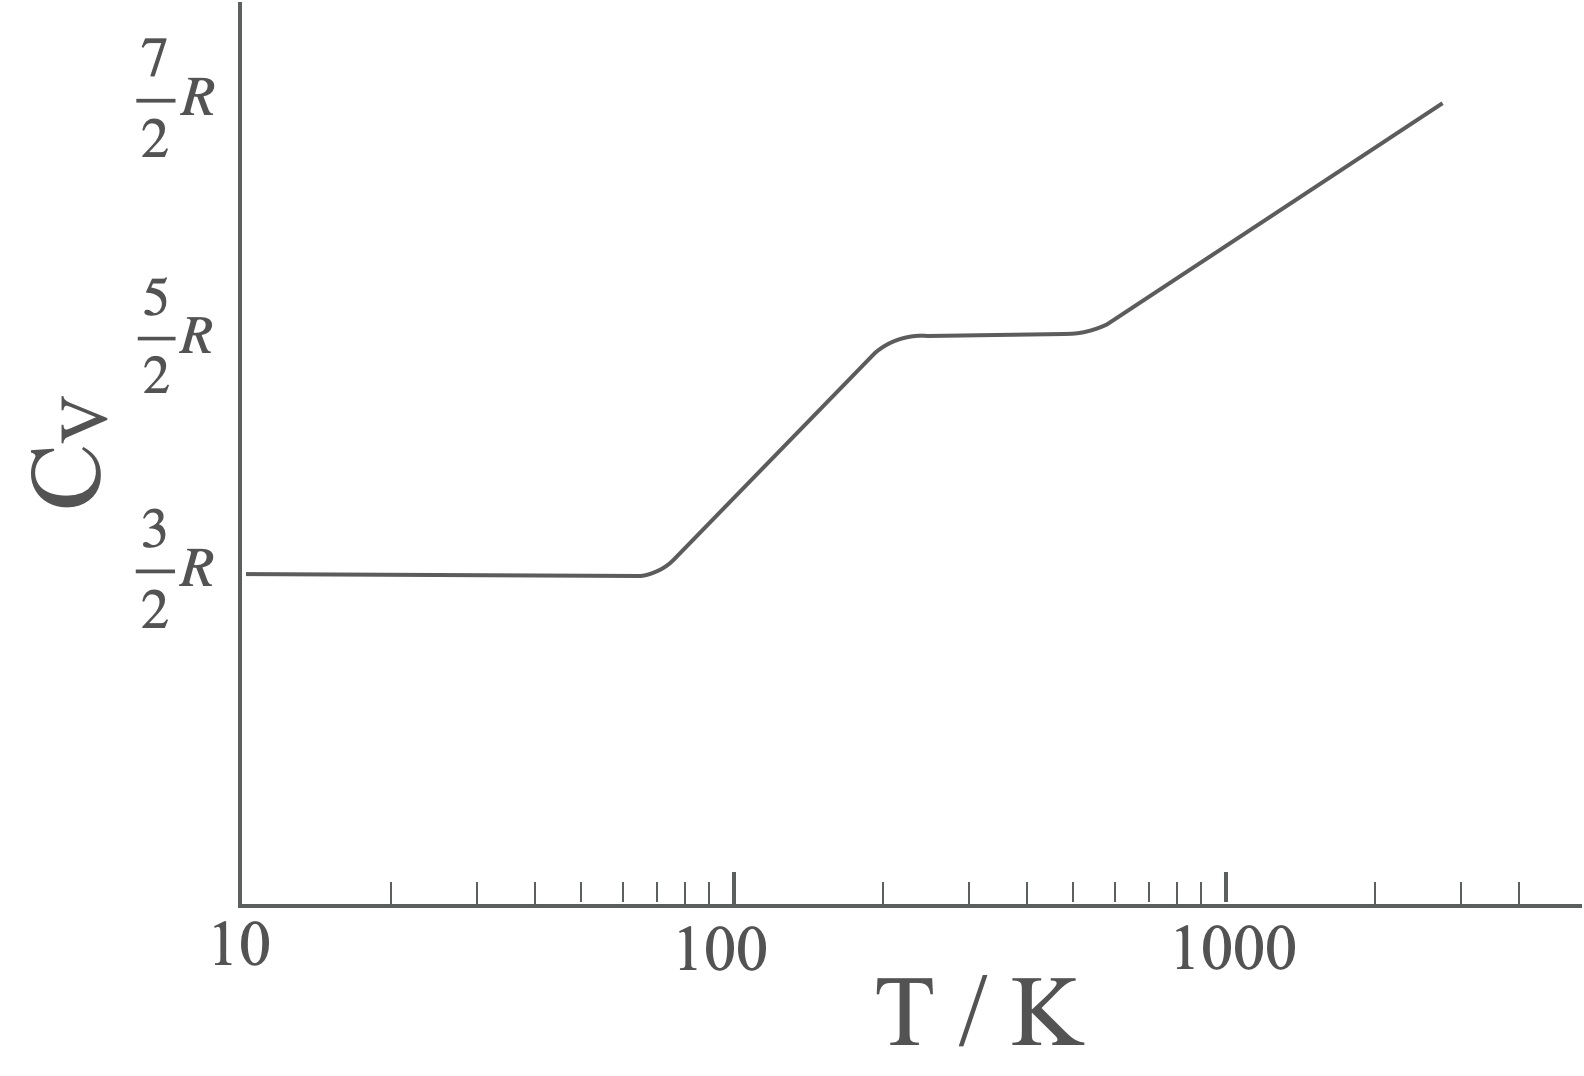
\includegraphics[width=0.7\linewidth]{images/H2heatcapacity} 

}

\caption{The heat capacity of molecular hydrogen varies with temperature, showing clear steps as each type of degree of freedom are activated. At very high temperatures dissociation occurs before the final plateau is observed.}\label{fig:H2heatcapacity}
\end{figure}

\hypertarget{temperature-dependance-of-enthalpy}{%
\section{Temperature dependance of enthalpy}\label{temperature-dependance-of-enthalpy}}

The enthalpy of reaction is dependent upon the temperature of reaction (figure \ref{fig:enthalpytemp}), the relationship between the enthalpies at two tempeartures are given in equation \ref{ed:kirchoff}. Standard enthalpies of fromation are defined usually at exactly 25 ºC.

\begin{equation}
\Delta_r H^{\ominus} (T')=\Delta_r H^{\ominus} (T) + \Delta_r C_p^{\ominus} (T'-T)
(eq:kirchoff)
\end{equation}

\begin{figure}

{\centering 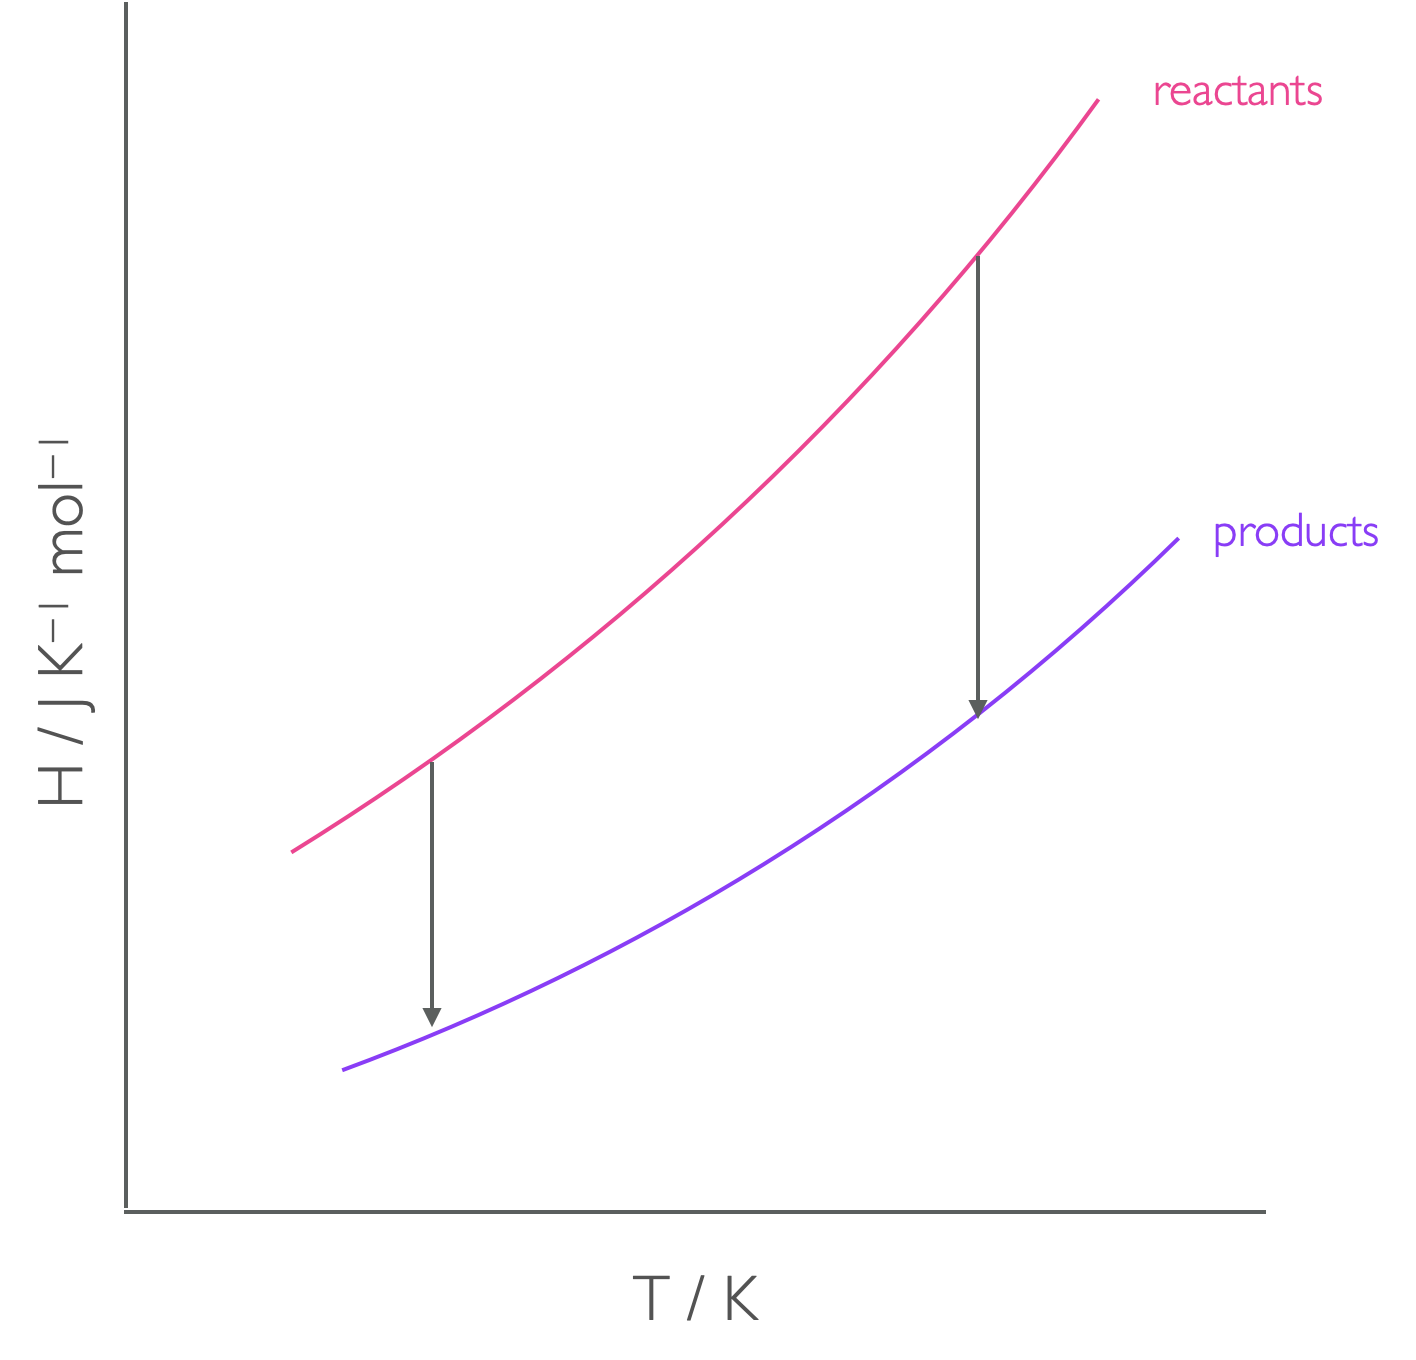
\includegraphics[width=0.7\linewidth]{images/enthalpytemp} 

}

\caption{The enthalpy of reaction is the difference in enthalpy between reactants and products, but this is tempearture dependant.}\label{fig:enthalpytemp}
\end{figure}

The value \(\Delta_r C_p^{\ominus}\) is the difference in heat capacity of the products and reactants at constant pressure. You have already seen this equation in equation \eqref{eq:heatcapacitystate} in section \ref{sec:equations1}.

For moderate changes in temperature we can assume that the heat capacity is a linear function and we can use Kirchoff's law (equation \eqref{eq:kirchoff}), but at larger temperature differences this function should really be integrated to account for the temperature dependance of heat capacity.

\hypertarget{enthalpy-of-phase-changes}{%
\section{Enthalpy of phase changes}\label{enthalpy-of-phase-changes}}

You are no doubt already familiar with the concepts of phase changes, and they are an increadibly important concept in thermodynamics which I will cover more than once during this course.

As energy in the form of heat is added to a system the temperature of that system usually increases, however there are some points where heat is added, but the temperature doesn't rise. However, at these points there is a distinct change in phase. This occurs no matter what two phases are involved.

The enthalpy of the phase change is a measure of the energy required (or released) when the intermolecular bonds between the molecules are broken or changed. Since transitions from the liquid to the gas phase involve complete breaking of the intermolecular bond enthalpies of fusion are always smaller than enthalpies of vapourisation.

\begin{figure}

{\centering 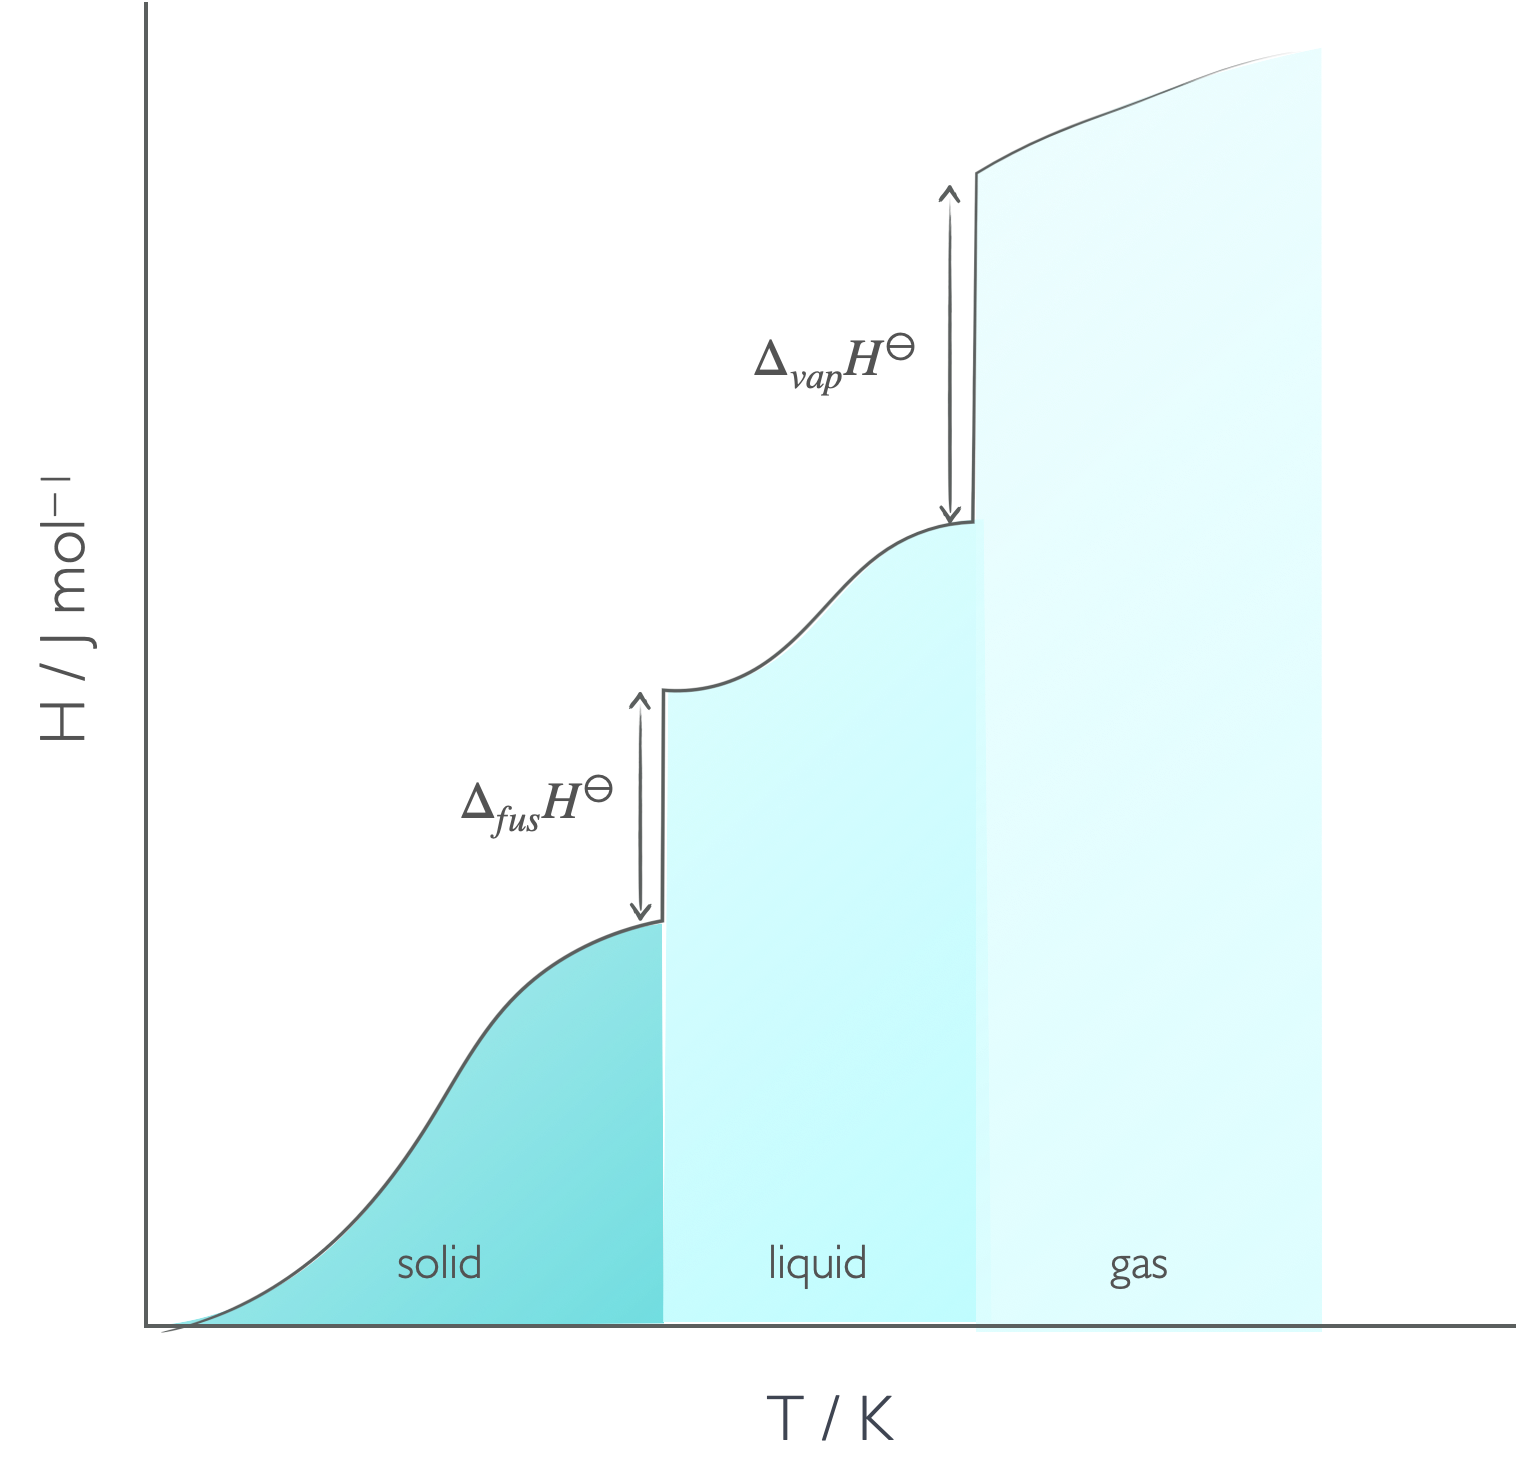
\includegraphics[width=0.7\linewidth]{images/enthalpyphasechange} 

}

\caption{As heat is added to the system usually the temperature increases, but there are points where heat is added but there is no increase in temperature, but instead a phase change.}\label{fig:enthalpyphasechange}
\end{figure}

We will meet phase changes later in the course when we consider both enthalpy and Gibbs' free energy so this is intentially just a very quick introduction.

\hypertarget{questions}{%
\section{Questions}\label{questions}}

\begin{enumerate}
\def\labelenumi{\arabic{enumi}.}
\item
  The constant pressure specific heat capacity of copper is 0.3850 kJ kg\textsuperscript{--1} K\textsuperscript{--1} at 298 K. Calculate the constant pressure heat capacity of 0.559 mol of copper at this temperature.
\item
  The constant pressure molar heat capacity of methane, CH\textsubscript{4}, is 35.31 J K\textsuperscript{--1} mol\textsuperscript{--1} at temperatures close to 298 K. Calculate the enthalpy change when 4.7 mol of methane is heated from a temperature of 266 K to 302 K.
\item
  What is the enthalpy of formation of water at 100 ºC if \(\Delta H_f = -241.82\) kJ mol\(^{-1}\) at 25 ºC? What assumptions have you made?
\end{enumerate}

c\(_{p,m} H_2 O = 33.58\) J K\(^{-1}\) mol\(^{-1}\)

c\(_{p,m} H_2 = 28.84\) J K\(^{-1}\) mol\(^{-1}\)

c\(_{p,m} O_2 = 29.37\) J K\(^{-1}\) mol\(^{-1}\)

\begin{enumerate}
\def\labelenumi{\arabic{enumi}.}
\setcounter{enumi}{3}
\tightlist
\item
  The complete combustion of ethane (C\textsubscript{2}H\textsubscript{6}) releases 1558.8 kJ mol\textsuperscript{−1} at 25 ºC. Calculate the enthalpy of combustion at 90 ºC.
\end{enumerate}

\begin{longtable}[]{@{}cc@{}}
\toprule
& C\textsubscript{p} / J K\textsuperscript{−1} mol\textsuperscript{−1}\tabularnewline
\midrule
\endhead
C\textsubscript{2}H\textsubscript{6} & 52.6\tabularnewline
O\textsubscript{2} & 29.4\tabularnewline
CO\textsubscript{2} & 37.1\tabularnewline
H\textsubscript{2}O & 75.3\tabularnewline
\bottomrule
\end{longtable}

\begin{enumerate}
\def\labelenumi{\arabic{enumi}.}
\setcounter{enumi}{4}
\tightlist
\item
  Calculate the enthalpy of formation of liquid mercury at 0 ºC. (C\textsubscript{p} = 27.98 J K\textsuperscript{−1} mol\textsuperscript{−1})

  \hypertarget{answers}{%
  \section{Answers}\label{answers}}
\item
  c = 13.7 J K\textsuperscript{--1}
\item
  ΔH = 6.0 kJ
\item
  \(\Delta _f H _{(\textrm{100 ºC})}=\) -242.57 kJ mol\textsuperscript{−1}
\item
  ΔH\textsubscript{363K} = -1549.4 kJ mol\textsuperscript{−1}
\item
  Δ\textsubscript{f}H\textsubscript{273K} = 0 kJ mol\textsuperscript{−1}
\end{enumerate}

\hypertarget{glossary-of-terms}{%
\chapter*{Glossary of terms}\label{glossary-of-terms}}
\addcontentsline{toc}{chapter}{Glossary of terms}

\hypertarget{a-f}{%
\section*{A-F}\label{a-f}}
\addcontentsline{toc}{section}{A-F}

\begin{itemize}
\item
  Adiabatic system: An adiabatic system can have no exchange of matter, and energy can only be exchanged in the form of work between the system and surroundings
\item
  Closed system: A closed system is one where there can be no exchnage of matter, but energy in either the form of heat or work may be exchanged between the system and surroundings.
\item
  Endothermic: an endothermic reaction has a positive value for ΔH and energy is transferred from the surroundings to the system in the form of heat
\item
  Exothermic: an exothermic reaction has a negative value for ΔH and energy is transferred from the system to the surroundings in the form of heat
\item
  Extensive property: a property which is dependent upon the amount of `stuff' you have, such as mass, volume, and enthalpy.
\end{itemize}

\hypertarget{g-m}{%
\section*{G-M}\label{g-m}}
\addcontentsline{toc}{section}{G-M}

\begin{itemize}
\item
  Heat: a mode of transfer of energy which causes chaotic (or non-uniform) motion of the system or surroundings
\item
  Heat capacity: see specific heat capacity or molar heat capacity
\item
  Intensive property: a property which is independent of the amount of `stuff' you have, such as temperature, molar volume, and molar enthalpy.
\item
  Isobaric: at constant pressure.
\item
  Isochoric: at constant thermal.
\item
  Isolated system: An isolated system is one where there can be no exchange of either matter or energy between the system and surroundings
\item
  Isothermal: at constant temperature.
\item
  Molar heat capacity: the energy in the form of heat requred to raise the temperature of 1 mol of a substance by 1 K
\end{itemize}

\hypertarget{n-s}{%
\section*{N-S}\label{n-s}}
\addcontentsline{toc}{section}{N-S}

\begin{itemize}
\item
  Open system: In an open system both matter and energy may be exchanged between the system and surroundings.
\item
  Path function: a path function is one which depends upon the route taken to go between the initial and final states. Functions such as work are path functions.
\item
  reversible: when a process is reversible in thermodynamics it is in equilibrium at all times and any changes which occur are infinitessimally small.
\item
  Specific heat capacity: the energy in the form of heat requred to raise the temperature of 1 kg (or 1 g) of a substance by 1 K
\item
  State function: a state function is one where only the current state of the system matters, for functions such as enthalpy change we only need to know the initial and final states and not how it got between those states.
\end{itemize}

\hypertarget{t-z}{%
\section*{T-Z}\label{t-z}}
\addcontentsline{toc}{section}{T-Z}

\begin{itemize}
\tightlist
\item
  Work: a mode of transfer of energy which causes uniform motion of the system or surroundings
\end{itemize}

  \bibliography{book.bib,packages.bib}

\end{document}
